\documentclass{article}

\usepackage{arxiv}

\usepackage[utf8]{inputenc} % allow utf-8 input
\usepackage[T1]{fontenc}    % use 8-bit T1 fonts
\usepackage{lmodern}        % https://github.com/rstudio/rticles/issues/343
\usepackage{hyperref}       % hyperlinks
\usepackage{url}            % simple URL typesetting
\usepackage{booktabs}       % professional-quality tables
\usepackage{amsfonts}       % blackboard math symbols
\usepackage{nicefrac}       % compact symbols for 1/2, etc.
\usepackage{microtype}      % microtypography
\usepackage{graphicx}

\title{Wrangling multivariate spatio-temporal data with the R package cubble}

\author{
    H. Sherry Zhang
   \\
    Monash University \\
  21 Chancellors Walk, Clayton VIC 3800 Australia \\
  \texttt{\href{mailto:huize.zhang@monash.edu}{\nolinkurl{huize.zhang@monash.edu}}} \\
   \And
    Dianne Cook
   \\
    Monash University \\
  21 Chancellors Walk, Clayton VIC 3800 Australia \\
  \texttt{\href{mailto:dicook@monash.edu}{\nolinkurl{dicook@monash.edu}}} \\
   \And
    Ursula Laa
   \\
    University of Natural Resources and Life Sciences \\
  Gregor-Mendel-Straße 33, 1180 Wien, Austria \\
  \texttt{\href{mailto:ursula.laa@boku.ac.at}{\nolinkurl{ursula.laa@boku.ac.at}}} \\
   \And
    Nicolas Langrené
   \\
    BNU-HKBU United International College \\
  2000 Jintong Road, Tangjiawan, Zhuhai, Guangdong Province, China \\
  \texttt{\href{mailto:nicolaslangrene@uic.edu.cn}{\nolinkurl{nicolaslangrene@uic.edu.cn}}} \\
   \And
    Patricia Menéndez
   \\
    Monash University \\
  21 Chancellors Walk, Clayton VIC 3800 Australia \\
  \texttt{\href{mailto:patricia.menendez@monash.edu}{\nolinkurl{patricia.menendez@monash.edu}}} \\
  }

% Pandoc syntax highlighting
\usepackage{color}
\usepackage{fancyvrb}
\newcommand{\VerbBar}{|}
\newcommand{\VERB}{\Verb[commandchars=\\\{\}]}
\DefineVerbatimEnvironment{Highlighting}{Verbatim}{commandchars=\\\{\}}
% Add ',fontsize=\small' for more characters per line
\usepackage{framed}
\definecolor{shadecolor}{RGB}{248,248,248}
\newenvironment{Shaded}{\begin{snugshade}}{\end{snugshade}}
\newcommand{\AlertTok}[1]{\textcolor[rgb]{0.94,0.16,0.16}{#1}}
\newcommand{\AnnotationTok}[1]{\textcolor[rgb]{0.56,0.35,0.01}{\textbf{\textit{#1}}}}
\newcommand{\AttributeTok}[1]{\textcolor[rgb]{0.77,0.63,0.00}{#1}}
\newcommand{\BaseNTok}[1]{\textcolor[rgb]{0.00,0.00,0.81}{#1}}
\newcommand{\BuiltInTok}[1]{#1}
\newcommand{\CharTok}[1]{\textcolor[rgb]{0.31,0.60,0.02}{#1}}
\newcommand{\CommentTok}[1]{\textcolor[rgb]{0.56,0.35,0.01}{\textit{#1}}}
\newcommand{\CommentVarTok}[1]{\textcolor[rgb]{0.56,0.35,0.01}{\textbf{\textit{#1}}}}
\newcommand{\ConstantTok}[1]{\textcolor[rgb]{0.00,0.00,0.00}{#1}}
\newcommand{\ControlFlowTok}[1]{\textcolor[rgb]{0.13,0.29,0.53}{\textbf{#1}}}
\newcommand{\DataTypeTok}[1]{\textcolor[rgb]{0.13,0.29,0.53}{#1}}
\newcommand{\DecValTok}[1]{\textcolor[rgb]{0.00,0.00,0.81}{#1}}
\newcommand{\DocumentationTok}[1]{\textcolor[rgb]{0.56,0.35,0.01}{\textbf{\textit{#1}}}}
\newcommand{\ErrorTok}[1]{\textcolor[rgb]{0.64,0.00,0.00}{\textbf{#1}}}
\newcommand{\ExtensionTok}[1]{#1}
\newcommand{\FloatTok}[1]{\textcolor[rgb]{0.00,0.00,0.81}{#1}}
\newcommand{\FunctionTok}[1]{\textcolor[rgb]{0.00,0.00,0.00}{#1}}
\newcommand{\ImportTok}[1]{#1}
\newcommand{\InformationTok}[1]{\textcolor[rgb]{0.56,0.35,0.01}{\textbf{\textit{#1}}}}
\newcommand{\KeywordTok}[1]{\textcolor[rgb]{0.13,0.29,0.53}{\textbf{#1}}}
\newcommand{\NormalTok}[1]{#1}
\newcommand{\OperatorTok}[1]{\textcolor[rgb]{0.81,0.36,0.00}{\textbf{#1}}}
\newcommand{\OtherTok}[1]{\textcolor[rgb]{0.56,0.35,0.01}{#1}}
\newcommand{\PreprocessorTok}[1]{\textcolor[rgb]{0.56,0.35,0.01}{\textit{#1}}}
\newcommand{\RegionMarkerTok}[1]{#1}
\newcommand{\SpecialCharTok}[1]{\textcolor[rgb]{0.00,0.00,0.00}{#1}}
\newcommand{\SpecialStringTok}[1]{\textcolor[rgb]{0.31,0.60,0.02}{#1}}
\newcommand{\StringTok}[1]{\textcolor[rgb]{0.31,0.60,0.02}{#1}}
\newcommand{\VariableTok}[1]{\textcolor[rgb]{0.00,0.00,0.00}{#1}}
\newcommand{\VerbatimStringTok}[1]{\textcolor[rgb]{0.31,0.60,0.02}{#1}}
\newcommand{\WarningTok}[1]{\textcolor[rgb]{0.56,0.35,0.01}{\textbf{\textit{#1}}}}

% tightlist command for lists without linebreak
\providecommand{\tightlist}{%
  \setlength{\itemsep}{0pt}\setlength{\parskip}{0pt}}

% From pandoc table feature
\usepackage{longtable,booktabs,array}
\usepackage{calc} % for calculating minipage widths
% Correct order of tables after \paragraph or \subparagraph
\usepackage{etoolbox}
\makeatletter
\patchcmd\longtable{\par}{\if@noskipsec\mbox{}\fi\par}{}{}
\makeatother
% Allow footnotes in longtable head/foot
\IfFileExists{footnotehyper.sty}{\usepackage{footnotehyper}}{\usepackage{footnote}}
\makesavenoteenv{longtable}

% Pandoc citation processing
\newlength{\cslhangindent}
\setlength{\cslhangindent}{1.5em}
\newlength{\csllabelwidth}
\setlength{\csllabelwidth}{3em}
\newlength{\cslentryspacingunit} % times entry-spacing
\setlength{\cslentryspacingunit}{\parskip}
% for Pandoc 2.8 to 2.10.1
\newenvironment{cslreferences}%
  {}%
  {\par}
% For Pandoc 2.11+
\newenvironment{CSLReferences}[2] % #1 hanging-ident, #2 entry spacing
 {% don't indent paragraphs
  \setlength{\parindent}{0pt}
  % turn on hanging indent if param 1 is 1
  \ifodd #1
  \let\oldpar\par
  \def\par{\hangindent=\cslhangindent\oldpar}
  \fi
  % set entry spacing
  \setlength{\parskip}{#2\cslentryspacingunit}
 }%
 {}
\usepackage{calc}
\newcommand{\CSLBlock}[1]{#1\hfill\break}
\newcommand{\CSLLeftMargin}[1]{\parbox[t]{\csllabelwidth}{#1}}
\newcommand{\CSLRightInline}[1]{\parbox[t]{\linewidth - \csllabelwidth}{#1}\break}
\newcommand{\CSLIndent}[1]{\hspace{\cslhangindent}#1}

\begin{document}
\maketitle


\begin{abstract}
Multivariate spatio-temporal data refers to multiple measurements taken across space and time. For many analyses, spatial and time components can be separately studied: for example, to explore the temporal trend of one variable for a single spatial location, or to model the spatial distribution of one variable at a given time. However for some studies, it is important to analyse different aspects of the spatio-temporal data simultaneouly, like for instance, temporal trends of multiple variables across locations. In order to facilitate the study of different portions or combinations of spatio-temporal data, we introduce a new data structure, \code{cubble}, with a suite of functions enabling easy slicing and dicing on the different components spatio-temporal components. The proposed \code{cubble} structure ensures that all the components of the data are easy to access and manipulate while providing flexibility for data analysis. In addition, \code{cubble} facilitates visual and numerical explorations of the data while easing data wrangling and modelling. The \code{cubble} structure and the functions provided in the \code{cubble} R package equip users with the capability to handle hierarchical spatial and temporal structures. The \code{cubble} structure and the tools implemented in the package are illustrated with different examples of Australian climate data.
\end{abstract}

\keywords{
    spatial, temporal, spatio temporal, R, exploratory data analysis, environmental data, climate data
  }

\newpage

\hypertarget{introduction}{%
\section{Introduction}\label{introduction}}

Spatio-temporal data has a spatial component referring to the location of each observation and a temporal component that is recorded at regular or irregular time intervals. It may also include multiple variables measured at each spatial and temporal values. With spatio-temporal data, one can fix the time to explore the spatial features of the data, fix the spatial location/s to explore temporal aspects, or dynamically explore the space and time simultaneously.
In order to computationally explore the spatial, temporal and spatio-temporal faces of such data, the data needs to be stored and represented under a specific data object that allows the user to query, group and dissect all the data faces.

The SpatioTemporal CRAN task view (\protect\hyperlink{ref-ctvspatiotemporal}{Edzer Pebesma 2022}) gathers information about R packages designed for spatio-temporal data and it has a section on \emph{Representing data} that lists existing spatio-temporal data representations used in \proglang{R}. Among them, E. Pebesma (\protect\hyperlink{ref-spacetime}{2012}) summarises spatio-temporal data into three forms: time-wide, space-wide, and long formats. The associated package \pkg{spacetime} (\protect\hyperlink{ref-spacetime}{E. Pebesma 2012}) implements four spatio-temporal layouts (full grid, sparse grid, irregular, and trajectory) to handle different space and time combinations. The \pkg{stars} (\protect\hyperlink{ref-stars}{E. Pebesma 2021}) package has a new implementation to use dense arrays to represent spatio-temporal cubes. It also interfaces with \pkg{sf} (\protect\hyperlink{ref-sf}{E. J. Pebesma 2018}), a package commonly used for wrangling spatial data, and the \pkg{tidyverse} (\protect\hyperlink{ref-tidyverse}{Wickham et al. 2019}) suite for general data wrangling and visualisation in \proglang{R}.

Still, the data representation for spatio-temporal data can be further extended and there are two reasons for this. Firstly, the raw data sourced in the wild is less often presented in any one of the layouts above, and fitting the raw data into a data object can sometimes be difficult. More often, spatio-temporal data are collected in separate 2D tables and analysts need to assemble them into a whole piece before exploring the data. Examples of components of spatio-temporal data can be 1) areal data recording the shape of a collection of areas of interest; 2) geostatistical data storing the longitude and latitude coordinates of locations, typically also with other metadata related to the location, and; 3) temporal data of each location across time.

The other reason is about tidy data concepts (\protect\hyperlink{ref-tidydata}{Wickham 2014}) and how they should be applied to spatio-temporal data. According to the tidy data principles, data should be structured into 1) one row per observation, 2) one column per variable, and 3) one type of data per table. The long form data is preferred over wide data form given the downstream software such as \pkg{dplyr} (\protect\hyperlink{ref-dplyr}{Wickham et al. 2022}) and \pkg{ggplot2} (\protect\hyperlink{ref-ggplot2}{Wickham 2016}) for data wrangling and visualisation. However, the long form can be inefficient to store feature geometries, especially for large multipolygons for hourly, daily or sub-daily periods over years, which are extensively collected and handled, for example in time series analysis. This poses the question of how to arrange spatial and temporal variables in a way that would make data wrangling, visualizing and analysing spatio-temporal data easier.

This paper presents a new \proglang{R} package, \pkg{cubble} which addresses the two issues mentioned above. In the package, a new data structure, also called \code{cubble}, is proposed to organise spatial and temporal variables as two forms of a single data object so that they can be wrangled separately or combined while being kept synchronised. Among the four spacetime layouts in E. Pebesma (\protect\hyperlink{ref-spacetime}{2012}), \pkg{cubble} can be applied to full grid, sparse grid, or irregular, but not trajectory, which is outside the scope of this work. The software is available from the Comprehensive R Archive Network (CRAN) at \url{https://CRAN.R-project.org/package=cubble}.

The rest of the paper is organized as follows: Section \ref{cube} introduces the proposed cube structure as a way to conceptualise multivariate spatio-temporal data. Section \ref{cubble} presents the main design and functionality of \pkg{cubble}. Section \ref{others} explains how cubble deals with more advanced considerations, including data with hierarchical structure, data matching and how cubble fits with existing static and interactive visualisation tools. Moreover we also illustrate how \pkg{cubble} deals with spatio-temporal data transformations. Section \ref{examples} uses Australian weather station data and river level data as examples to demonstrate the use of \pkg{cubble}. An example of how \pkg{cubble} handles NetCDF data is also provided. Section \ref{conclude} discuss the paper contributions and future directions.

\hypertarget{cube}{%
\section{Conceptual framework: spatio-temporal cube}\label{cube}}

Spatio-temporal data can be conceptualised using a cubical data model with three axes which typically are, time, latitude and longitude. This abstraction can be useful for generalising operations and visualisation purposes: Lu, Appel, and Pebesma (\protect\hyperlink{ref-lu_multidimensional_2018}{2018}) shows how array operations (select, scale, reduce, rearrange, and compute) can be mapped onto the cube; Bach et al. (\protect\hyperlink{ref-bach_review_2014}{2014}) reviews the temporal data visualisation based on space-time cube operations. Notice that the term space-time cube in their article ``does not need to involve spatial data'', but refers to ``an abstract 2D substrate that is used to visualize data at a specific time''. Despite its main focus being on temporal data, the mindset of abstracting out data representation to construct visualisations, still applies to our spatio-temporal data manipulation and visualisation approaches.

The most common data cube using the three axes (time, latitude, longitude) could be considered as taking snapshots of the space and stacking them across time. Here we define the spatio-temporal cube slightly differently by considering the three axes to be, time, site and variable/s. That is illustrated in the leftmost cube in Figure \ref{fig:cube-def}. The time axis is the same in both versions, while the site axis now captures both latitude and longitude. Finally, variables are stacked on this space-time canvas, with one observation per site and time point. This notion is adopted to avoid using hypercubes when describing multivariate spatio-temporal data and is the conceptual framework behind \pkg{cubble}. With this conceptual model, operations on spatio-temporal data can be mapped to operations on the cube and the rest of Figure \ref{fig:cube-def} show examples of slicing on site, time, and variable.

While a cubical data model is neat to view spatio-temporal data conceptually, a 3D data representation, or an array, may not be convenient for data wrangling. There are two reasons for this: 1) While arrays are efficient for the computation on numerical values, spatio-temporal data, in general, contains more than just numerical variables. For example, wrangling on character strings and specific datetime classes is common for spatio-temporal data but may not be easily done with array objects. 2) Creating new variables in an array is more complex than in a data frame since it would need to be defined in a 2D space, rather than a 1D vector, to be added into the array.

\begin{figure}

{\centering 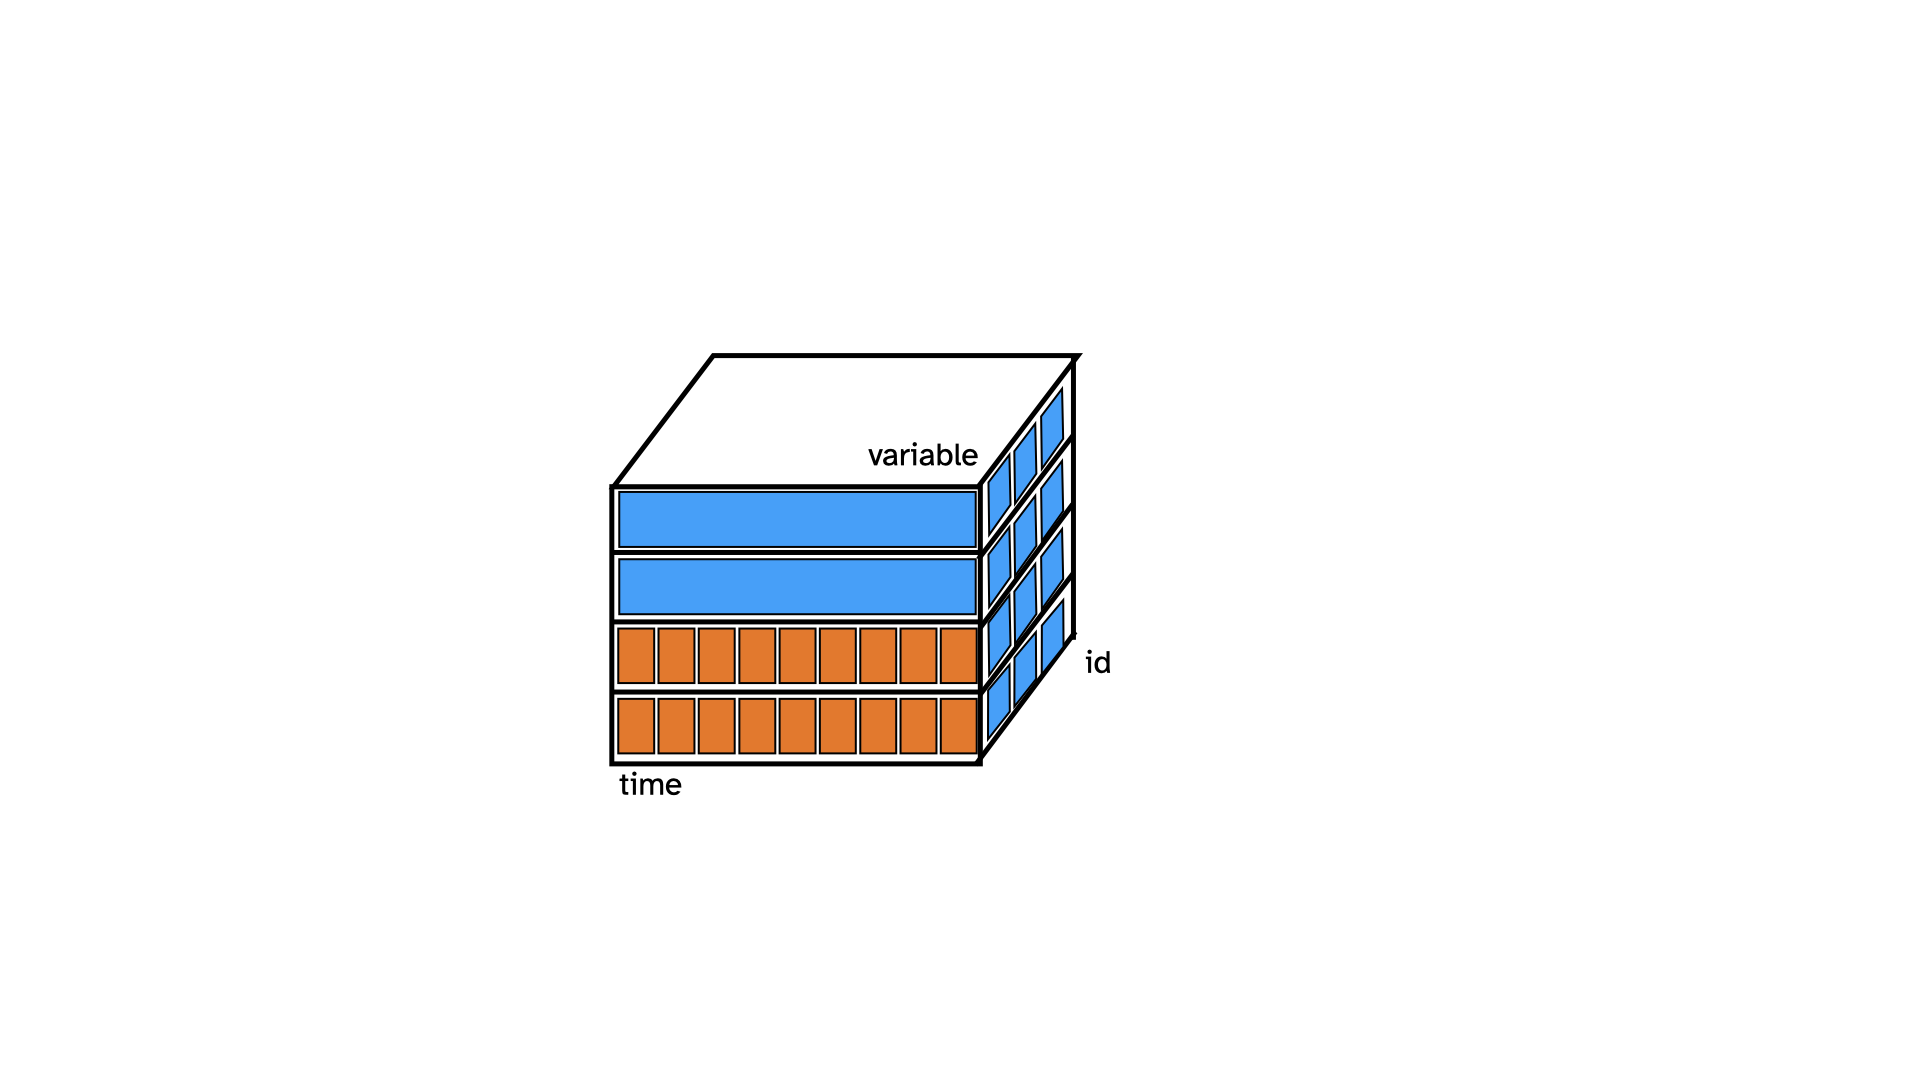
\includegraphics[width=1\linewidth]{/Users/sherryzhang/Documents/research/paper-cubble/figures/diagram-keynotes/diagram-keynotes.007} 

}

\caption{An illustration of the conceptual spatio-temporal cube with different slicing on time, site, and variable. For each axis, the slicing can be on a single value or a set of values.}\label{fig:cube-def}
\end{figure}

\hypertarget{cubble}{%
\section{The cubble package}\label{cubble}}

Here we introduce the core functionalities of cubble. The main functions, \code{as_cubble()}, \code{face_spatial()}, \code{face_temporal()}, and \code{unfold()} are described in Section \ref{create} - \ref{unfold}. Section \ref{tidyverse} explains the need to create a new class. Section \ref{compact} will then discusses how cubble relates to existing packages for spatial and temporal data analysis.

The dataset \texttt{climate\_flat} is used to illustrate \pkg{cubble} functionality. This is a subset from the ORIGIN and contains the spatial variables, station id, latitude, longitude, elevation, station name, World Meteorology Organisation ID, in additional to daily temporal information, maximum and minimum temperature values and precipitation records for 2020. The first five rows of \texttt{climate\_flat} are shown below:

\begin{verbatim}
## # A tibble: 1,830 x 10
##   id            lat  long  elev name         wmo_id date        prcp  tmax  tmin
##   <chr>       <dbl> <dbl> <dbl> <chr>         <dbl> <date>     <dbl> <dbl> <dbl>
## 1 ASN00009021 -31.9  116.  15.4 perth airpo~  94610 2020-01-01     0  31.9  15.3
## 2 ASN00009021 -31.9  116.  15.4 perth airpo~  94610 2020-01-02     0  24.9  16.4
## 3 ASN00009021 -31.9  116.  15.4 perth airpo~  94610 2020-01-03     6  23.2  13  
## 4 ASN00009021 -31.9  116.  15.4 perth airpo~  94610 2020-01-04     0  28.4  12.4
## 5 ASN00009021 -31.9  116.  15.4 perth airpo~  94610 2020-01-05     0  35.3  11.6
## # ... with 1,825 more rows
\end{verbatim}

\hypertarget{create}{%
\subsection{Create a cubble}\label{create}}

A cubble can be created from various common spatio-temporal data formats, including basic R objects like tibble, tsibble, sf. Section \ref{covid} describes converting multiple tables into a cubble object and Section \ref{netcdf} illustrate how to convert a netCDF object.

The function \code{as_cubble()} is used to create a cubble with three arguments: \code{key} as the spatial identifier; \code{index} as the temporal identifier; and a vector of \code{coords} in the order (longitude, latitude). The arguments \code{key} and \code{index} follow the wording in \pkg{tsibble} to describe the temporal order and multiple series while \code{coords} specifies the spatial location of each site. The code below creates a cubble out of \code{climate_flat} (a single tibble) with \code{id} as the key, \code{date} as the index, and \code{c(long, lat)} as the coordinates:

\begin{Shaded}
\begin{Highlighting}[]
\NormalTok{cubble\_nested }\OtherTok{\textless{}{-}}\NormalTok{ climate\_flat }\SpecialCharTok{|\textgreater{}}
  \FunctionTok{as\_cubble}\NormalTok{(}\AttributeTok{key =}\NormalTok{ id, }\AttributeTok{index =}\NormalTok{ date, }\AttributeTok{coords =} \FunctionTok{c}\NormalTok{(long, lat))}
\NormalTok{cubble\_nested}
\end{Highlighting}
\end{Shaded}

\begin{verbatim}
## # cubble:   id [5]: nested form
## # bbox:     [115.97, -32.94, 133.55, -12.42]
## # temporal: date [date], prcp [dbl], tmax [dbl], tmin [dbl]
##   id            lat  long  elev name           wmo_id ts                
##   <chr>       <dbl> <dbl> <dbl> <chr>           <dbl> <list>            
## 1 ASN00009021 -31.9  116.  15.4 perth airport   94610 <tibble [366 x 4]>
## 2 ASN00010311 -31.9  117. 179   york            94623 <tibble [366 x 4]>
## 3 ASN00010614 -32.9  117. 338   narrogin        94627 <tibble [366 x 4]>
## 4 ASN00014015 -12.4  131.  30.4 darwin airport  94120 <tibble [366 x 4]>
## 5 ASN00015131 -17.6  134. 220   elliott         94236 <tibble [366 x 4]>
\end{verbatim}

Printing a cubble provides some information about the data. \code{id} is the variable name to identify each location and there are five unique locations. The bounding box is \code{[115.97, -32.94, 133.55, -12.42]} and provides information about the coordinates in the data set. The third row shows the name and type of all variables nested in the \code{ts} column. In this example, it includes \code{date [date], prcp [dbl], tmax [dbl], tmin [dbl]}.

A cubble object is an extension of a \code{rowwise_df} object where each row forms a group. All the temporal variables are nested in a list column, hence it is also called the nested cubble. The rowwise structure makes it simpler to operate on the list using the \code{mutate()} syntax, which is simpler than the \code{purr::map()} when working with a list column. For example, calculating the number of rainy days can be done by:

\begin{Shaded}
\begin{Highlighting}[]
\NormalTok{cubble\_nested }\SpecialCharTok{|\textgreater{}}
  \FunctionTok{mutate}\NormalTok{(}\AttributeTok{rain\_day =} \FunctionTok{sum}\NormalTok{(ts}\SpecialCharTok{$}\NormalTok{prcp }\SpecialCharTok{!=} \DecValTok{0}\NormalTok{))}
\end{Highlighting}
\end{Shaded}

\begin{verbatim}
## # cubble:   id [5]: nested form
## # bbox:     [115.97, -32.94, 133.55, -12.42]
## # temporal: date [date], prcp [dbl], tmax [dbl], tmin [dbl]
##   id            lat  long  elev name           wmo_id ts       rain_day
##   <chr>       <dbl> <dbl> <dbl> <chr>           <dbl> <list>      <int>
## 1 ASN00009021 -31.9  116.  15.4 perth airport   94610 <tibble>      104
## 2 ASN00010311 -31.9  117. 179   york            94623 <tibble>       89
## 3 ASN00010614 -32.9  117. 338   narrogin        94627 <tibble>       90
## 4 ASN00014015 -12.4  131.  30.4 darwin airport  94120 <tibble>      106
## 5 ASN00015131 -17.6  134. 220   elliott         94236 <tibble>       63
\end{verbatim}

\hypertarget{change-focus-by-facing-the-time-variables}{%
\subsection{Change focus by facing the time-variables}\label{change-focus-by-facing-the-time-variables}}

The nested form can be used for those operations where the output is only indexed by the spatial identifier (\code{key}), but becomes inadequate when outputs need both a spatial and a temporal identifier (\code{key} and \code{index}). The \pkg{cubble} class also provides a long form, which expands the \code{ts} column and temporarily ``hides'' the spatial variables. The function \code{face_temporal()} is used to switch from the nested cubble into the long one. The first row in Figure \ref{fig:face} illustrates this operation where the focus of the cube now changes from the site-variable face to the time-variable face. This code switches the cubble just created into its long form:

\begin{Shaded}
\begin{Highlighting}[]
\NormalTok{cubble\_long }\OtherTok{\textless{}{-}}\NormalTok{ cubble\_nested }\SpecialCharTok{|\textgreater{}} \FunctionTok{face\_temporal}\NormalTok{()}
\NormalTok{cubble\_long}
\end{Highlighting}
\end{Shaded}

\begin{verbatim}
## # cubble:  date, id [5]: long form
## # bbox:    [115.97, -32.94, 133.55, -12.42]
## # spatial: lat [dbl], long [dbl], elev [dbl], name [chr], wmo_id [dbl]
##   id          date        prcp  tmax  tmin
##   <chr>       <date>     <dbl> <dbl> <dbl>
## 1 ASN00009021 2020-01-01     0  31.9  15.3
## 2 ASN00009021 2020-01-02     0  24.9  16.4
## 3 ASN00009021 2020-01-03     6  23.2  13  
## 4 ASN00009021 2020-01-04     0  28.4  12.4
## 5 ASN00009021 2020-01-05     0  35.3  11.6
## # ... with 1,825 more rows
\end{verbatim}

The first line in printed cubble now shows the cubble in its long form and the third line has been changed to display the name and type of spatial variables: \code{lat [dbl], long [dbl], elev [dbl], name [chr], wmo_id [dbl]}. Unlike the nested form, the long cubble is built from a \code{grouped_df} object where all the observations from the same sites form a group.

\begin{figure}

{\centering 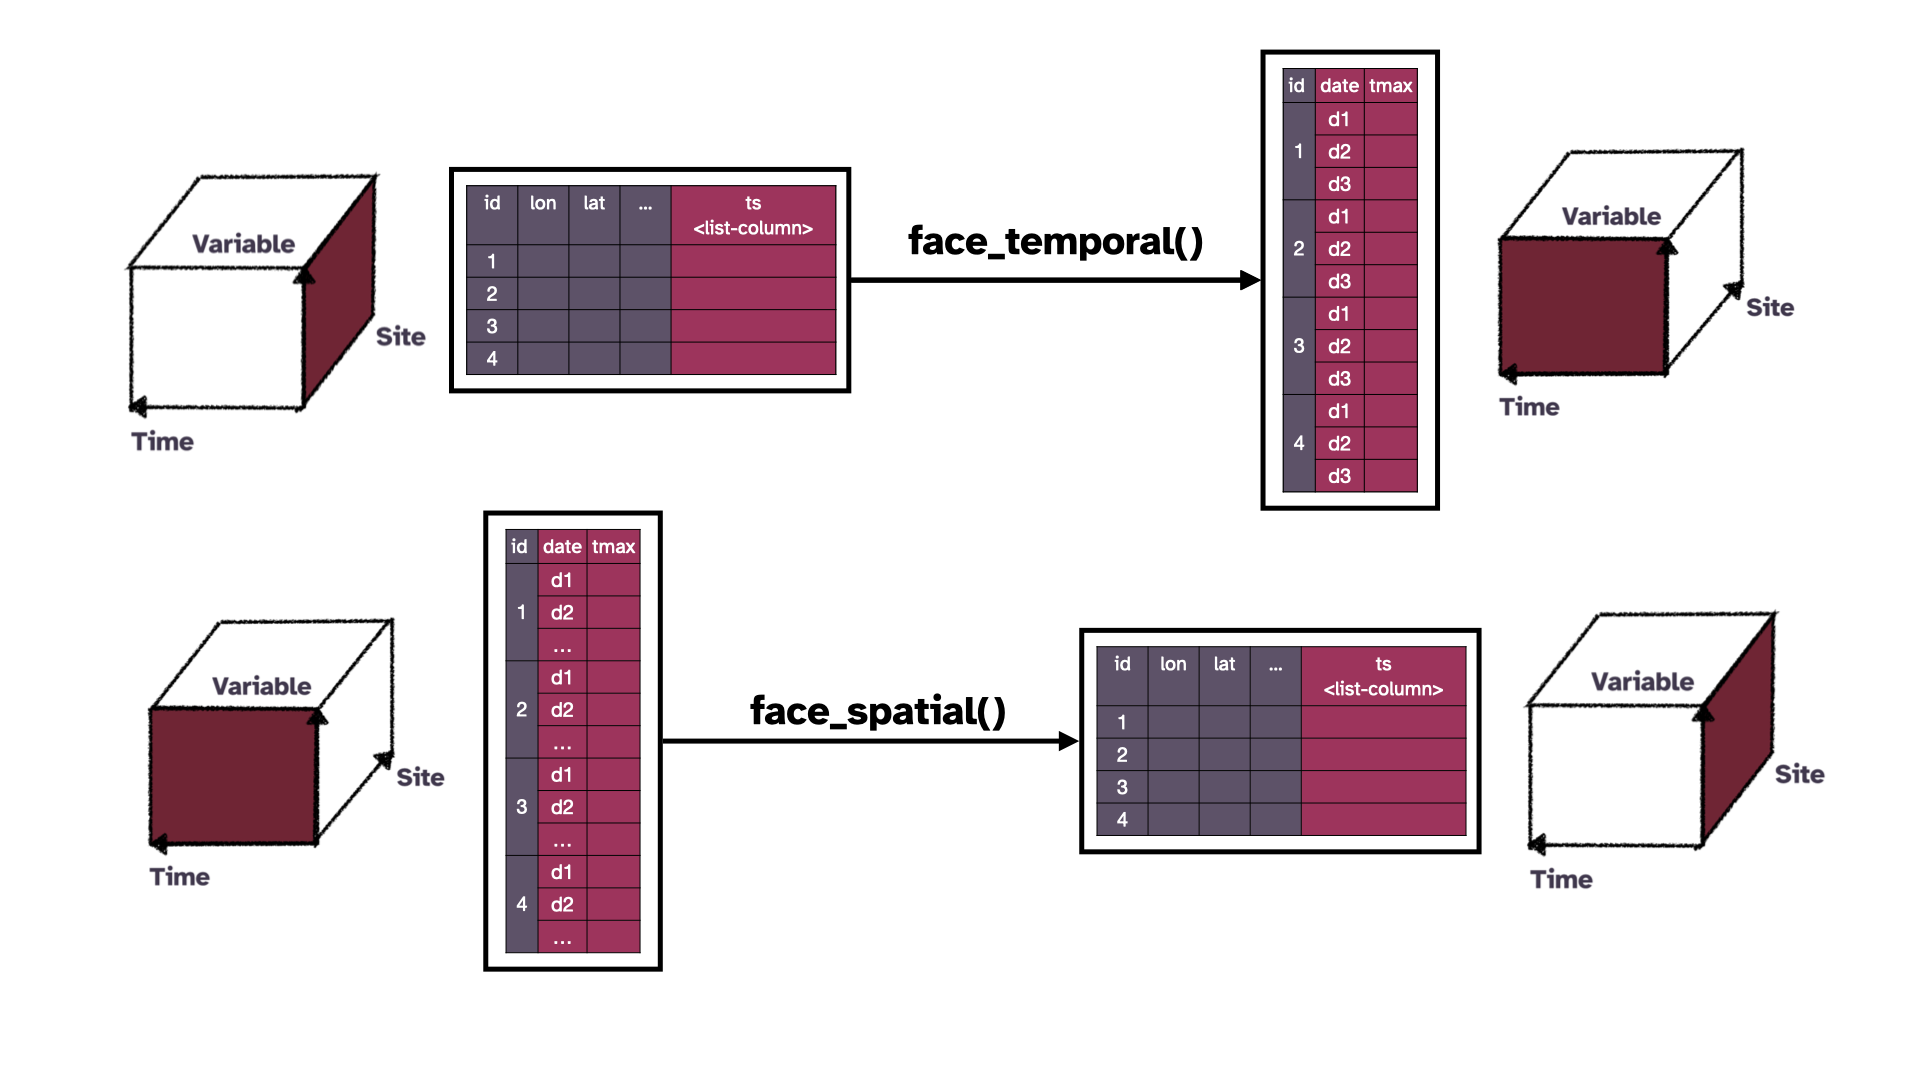
\includegraphics[width=1\linewidth]{/Users/sherryzhang/Documents/research/paper-cubble/figures/diagram-keynotes/diagram-keynotes.008} 

}

\caption{An illustration of function \code{face\_temporal} and \code{face\_spatial} in cubble. In the first row, \code{face\_temporal} switches a cubble from the nested form into the long form and the focus has switched from the spatial aspect (the side face) to the temporal aspect (the front face). In the second row, \code{face\_spatial} switches a cubble back to the nested form from the long form and shifts focus back to the spatial aspect.}\label{fig:face}
\end{figure}

\hypertarget{change-focus-back-to-the-site-variable-face}{%
\subsection{Change focus back to the site-variable face}\label{change-focus-back-to-the-site-variable-face}}

Wrangling spatio-temporal data can be seen as an iterative process in the spatial and temporal dimensions. Switching the focus back to the site-variable face can be accomplished by the function \code{face_spatial()}, which is the inverse of \code{face_temporal()}. The second row of Figure \ref{fig:face} illustrates the function, which is used as follows:

\begin{Shaded}
\begin{Highlighting}[]
\NormalTok{cubble\_back }\OtherTok{\textless{}{-}}\NormalTok{ cubble\_long }\SpecialCharTok{|\textgreater{}} \FunctionTok{face\_spatial}\NormalTok{()}
\NormalTok{cubble\_back}
\end{Highlighting}
\end{Shaded}

\begin{verbatim}
## # cubble:   id [5]: nested form
## # bbox:     [115.97, -32.94, 133.55, -12.42]
## # temporal: date [date], prcp [dbl], tmax [dbl], tmin [dbl]
##   id            lat  long  elev name           wmo_id ts                
##   <chr>       <dbl> <dbl> <dbl> <chr>           <dbl> <list>            
## 1 ASN00009021 -31.9  116.  15.4 perth airport   94610 <tibble [366 x 4]>
## 2 ASN00010311 -31.9  117. 179   york            94623 <tibble [366 x 4]>
## 3 ASN00010614 -32.9  117. 338   narrogin        94627 <tibble [366 x 4]>
## 4 ASN00014015 -12.4  131.  30.4 darwin airport  94120 <tibble [366 x 4]>
## 5 ASN00015131 -17.6  134. 220   elliott         94236 <tibble [366 x 4]>
\end{verbatim}

\begin{Shaded}
\begin{Highlighting}[]
\FunctionTok{identical}\NormalTok{(cubble\_nested, cubble\_back)}
\end{Highlighting}
\end{Shaded}

\begin{verbatim}
## [1] TRUE
\end{verbatim}

\hypertarget{unfold}{%
\subsection{Unfold spatial variables into the long cubble}\label{unfold}}

Sometimes, analysts may need to apply some variable transformation that involves both the spatial and temporal variables. An example of this is the transformation of temporal variables into the spatial dimension in glyph maps {[}ref{]}. (Glyph maps will be explained in Section \ref{st_transformation}.) This type of operation can be seen as flattening, or \emph{unfolding}, the cube into a 2D data frame. Here the function \code{unfold()} moves the spatial variables \code{long} and \code{lat} into the long cubble:

\begin{Shaded}
\begin{Highlighting}[]
\NormalTok{cubble\_unfold }\OtherTok{\textless{}{-}}\NormalTok{ cubble\_long }\SpecialCharTok{|\textgreater{}} \FunctionTok{unfold}\NormalTok{(long, lat)}
\NormalTok{cubble\_unfold}
\end{Highlighting}
\end{Shaded}

\begin{verbatim}
## # cubble:  date, id [5]: long form
## # bbox:    [115.97, -32.94, 133.55, -12.42]
## # spatial: lat [dbl], long [dbl], elev [dbl], name [chr], wmo_id [dbl]
##   id          date        prcp  tmax  tmin  long   lat
##   <chr>       <date>     <dbl> <dbl> <dbl> <dbl> <dbl>
## 1 ASN00009021 2020-01-01     0  31.9  15.3  116. -31.9
## 2 ASN00009021 2020-01-02     0  24.9  16.4  116. -31.9
## 3 ASN00009021 2020-01-03     6  23.2  13    116. -31.9
## 4 ASN00009021 2020-01-04     0  28.4  12.4  116. -31.9
## 5 ASN00009021 2020-01-05     0  35.3  11.6  116. -31.9
## # ... with 1,825 more rows
\end{verbatim}

This function should generally be used in the last step of the analysis since it is a temporary operation, meaning that these added spatial variables will disappear, if switched to the nested form and then switched back:

\begin{Shaded}
\begin{Highlighting}[]
\NormalTok{cubble\_unfold }\SpecialCharTok{|\textgreater{}} \FunctionTok{face\_spatial}\NormalTok{() }\SpecialCharTok{|\textgreater{}} \FunctionTok{face\_temporal}\NormalTok{()}
\end{Highlighting}
\end{Shaded}

\begin{verbatim}
## # cubble:  date, id [5]: long form
## # bbox:    [115.97, -32.94, 133.55, -12.42]
## # spatial: lat [dbl], long [dbl], elev [dbl], name [chr], wmo_id [dbl]
##   id          date        prcp  tmax  tmin
##   <chr>       <date>     <dbl> <dbl> <dbl>
## 1 ASN00009021 2020-01-01     0  31.9  15.3
## 2 ASN00009021 2020-01-02     0  24.9  16.4
## 3 ASN00009021 2020-01-03     6  23.2  13  
## 4 ASN00009021 2020-01-04     0  28.4  12.4
## 5 ASN00009021 2020-01-05     0  35.3  11.6
## # ... with 1,825 more rows
\end{verbatim}

\hypertarget{tidyverse}{%
\subsection{Why not just use the existing tidyverse functions}\label{tidyverse}}

Some readers may question why a new data structure is needed rather than using \code{dplyr::nest_by()} on the combined data to directly create a list-column. The reason is that cubble is specifically designed to utilize the spatio-temporal structure when arranging variables from different observational units into a single object. Moreover, it enables easy pivoting between purely spatial, purely temporal, or unfolded into a combined form.

\hypertarget{compact}{%
\subsection{Compatibility with existing packages}\label{compact}}

This section will demonstrate how the \code{cubble} class interacts with existing packages commonly used in spatial and temporal analysis, specifically, \code{dplyr}, \code{tsibble}, \code{sf} (\code{s2}), and \code{netcdf4}.

\hypertarget{dplyr}{%
\subsubsection{dplyr}\label{dplyr}}

The \code{dplyr} package has introduced many tools for data wrangling tasks and these operations are useful in the spatio-temporal context. \code{cubble} provides methods that support the following \code{dplyr} verbs in both the nested and long form:

\begin{quote}
\texttt{mutate}, \texttt{filter}, \texttt{summarise}, \texttt{select}, \texttt{arrange}, \texttt{rename}, \texttt{left\_join}, and the slice family (\texttt{slice\_head}, \texttt{slice\_tail}, \texttt{slice\_sample}, \texttt{slice\_min}, \texttt{slice\_max})
\end{quote}

\hypertarget{tsibble}{%
\subsubsection{tsibble}\label{tsibble}}

\code{tsibble} is a temporal data structure that uses \code{index} and \code{key} to identify the time and different series. \code{cubble} can be seen as following the same vein as \code{tsibble} for spatio-temporal data. This makes it easy to cast a \code{tsibble} into a \code{cubble} as only the \code{coords} argument needs to be supplied:

\begin{Shaded}
\begin{Highlighting}[]
\CommentTok{\# example with a tsibble created from climate\_flat}
\NormalTok{raw }\OtherTok{\textless{}{-}}\NormalTok{ climate\_flat }\SpecialCharTok{|\textgreater{}}\NormalTok{ tsibble}\SpecialCharTok{::}\FunctionTok{as\_tsibble}\NormalTok{(}\AttributeTok{key =}\NormalTok{ id, }\AttributeTok{index =}\NormalTok{ date)}
\NormalTok{dt }\OtherTok{\textless{}{-}}\NormalTok{  raw }\SpecialCharTok{|\textgreater{}}\NormalTok{ cubble}\SpecialCharTok{::}\FunctionTok{as\_cubble}\NormalTok{(}\AttributeTok{coords =} \FunctionTok{c}\NormalTok{(long, lat))}
\NormalTok{dt}
\end{Highlighting}
\end{Shaded}

\begin{verbatim}
## # cubble:   id [5]: nested form
## # bbox:     [115.97, -32.94, 133.55, -12.42]
## # temporal: date [date], prcp [dbl], tmax [dbl], tmin [dbl]
##   id            lat  long  elev name           wmo_id ts                
##   <chr>       <dbl> <dbl> <dbl> <chr>           <dbl> <list>            
## 1 ASN00009021 -31.9  116.  15.4 perth airport   94610 <tbl_ts [366 x 4]>
## 2 ASN00010311 -31.9  117. 179   york            94623 <tbl_ts [366 x 4]>
## 3 ASN00010614 -32.9  117. 338   narrogin        94627 <tbl_ts [366 x 4]>
## 4 ASN00014015 -12.4  131.  30.4 darwin airport  94120 <tbl_ts [366 x 4]>
## 5 ASN00015131 -17.6  134. 220   elliott         94236 <tbl_ts [366 x 4]>
\end{verbatim}

When a nested cubble is created, each element in the list-column \code{ts} is of \code{tbl_ts} class and operations available to the tsibble class are still valid within the cubble. For example, the code below calculates two time series features (mean and variance) of the maximum temperature variable:

\begin{Shaded}
\begin{Highlighting}[]
\CommentTok{\# add station{-}based features in the nested form.}
\NormalTok{dt }\SpecialCharTok{|\textgreater{}} \FunctionTok{mutate}\NormalTok{(fabletools}\SpecialCharTok{::}\FunctionTok{features}\NormalTok{(ts, tmax, }\FunctionTok{list}\NormalTok{(}\AttributeTok{tmax\_mean =}\NormalTok{ mean, }\AttributeTok{tmax\_var =}\NormalTok{ var)))}
\end{Highlighting}
\end{Shaded}

\begin{verbatim}
## # cubble:   id [5]: nested form
## # bbox:     [115.97, -32.94, 133.55, -12.42]
## # temporal: date [date], prcp [dbl], tmax [dbl], tmin [dbl]
##   id            lat  long  elev name          wmo_id ts       tmax_mean tmax_var
##   <chr>       <dbl> <dbl> <dbl> <chr>          <dbl> <list>       <dbl>    <dbl>
## 1 ASN00009021 -31.9  116.  15.4 perth airport  94610 <tbl_ts>      25.7    38.6 
## 2 ASN00010311 -31.9  117. 179   york           94623 <tbl_ts>      26.2    51.1 
## 3 ASN00010614 -32.9  117. 338   narrogin       94627 <tbl_ts>      23.7    45.4 
## 4 ASN00014015 -12.4  131.  30.4 darwin airpo~  94120 <tbl_ts>      33.1     3.02
## 5 ASN00015131 -17.6  134. 220   elliott        94236 <tbl_ts>      34.6    24.7
\end{verbatim}

\hypertarget{sf-and-s2}{%
\subsubsection{sf and s2}\label{sf-and-s2}}

As a spatial data object, \code{sf} creates a feature geometry list-column (\code{sfc}) in the data frame to provide spatial operations on various geometry types such as (\code{POINT}, \code{LINESTRING}, \code{POLYGON}, \code{MULTIPOLYGON}, etc). When creating a cubble a \code{sf} object can be supplied as the spatial table. Once that is included in a cubble, methods for the \code{sfc} class can be applied in the nested form inside the cubble object. An example of this is shown in \ref{covid}, which also handles the case when the site identifiers in the two tables do not match exactly. A spatial data object with an \code{s2} vector can also be the input for the spatial table in \pkg{cubble}.

\hypertarget{netcdf}{%
\subsubsection{netcdf}\label{netcdf}}

NetCDF data is another format that is commonly used for storing spatio-temporal data. It has two main components: \emph{dimension} for defining the spatio-temporal grid (longitude, latitude, and time) and \emph{variable} that populates the defined grid. Attributes are usually associated with dimensions and variables in the NetCDF format data and a \href{http://cfconventions.org/}{metadata convention for climate and forecast} has been designed to standardise the format of the attributes. A few packages in R exist for manipulating NetCDF data and these include a high-level R interface: \pkg{ncdf4} (\protect\hyperlink{ref-ncdf4}{Pierce 2019}), a low-level interface that calls a C-interface: \pkg{RNetCDF} (\protect\hyperlink{ref-rnetcdf}{Michna and Woods 2021}, \protect\hyperlink{ref-michna2013rnetcdf}{2013}), and a tidyverse implementation: \pkg{tidync} (\protect\hyperlink{ref-tidync}{Sumner 2020}).

Cubble provides an \code{as_cubble()} method to coerce the \code{ncdf4} class from the \pkg{ncdf4} package into a \code{cubble}. It maps each combination of longitude and latitude into an \code{id} as the \code{key}:

\begin{Shaded}
\begin{Highlighting}[]
\CommentTok{\# read in the .nc file as a ncdf4 class}
\NormalTok{raw }\OtherTok{\textless{}{-}}\NormalTok{ ncdf4}\SpecialCharTok{::}\FunctionTok{nc\_open}\NormalTok{(here}\SpecialCharTok{::}\FunctionTok{here}\NormalTok{(}\StringTok{"data/era5{-}pressure.nc"}\NormalTok{))}

\CommentTok{\# convert the variable q and z in the ncdf4 into a cubble}
\NormalTok{dt }\OtherTok{\textless{}{-}} \FunctionTok{as\_cubble}\NormalTok{(raw, }\AttributeTok{vars =} \FunctionTok{c}\NormalTok{(}\StringTok{"q"}\NormalTok{, }\StringTok{"z"}\NormalTok{))}
\end{Highlighting}
\end{Shaded}

The memory limit with NetCDF data in cubble depends on the number of longitude grid points \(\times\) the number of latitude grid points \(\times\) the number of time grid points \(\times\) the number of variables. Cubble can handle slightly more than 300 \(\times\) 300 (longitude \(\times\) longitude) grid points for three daily variables in one year. A 300 by 300 spatial grid can be a bounding box of {[}100, -80, 180, 0{]} at 0.25 degree resolution or a global bounding box {[}-180, -90, 180, -90{]} at 1 degree resolution. The spatial grid can also be subsetted to trade for longer time periods and more variables through \code{long_range} and \code{lat_range} if the NetCDF file has finer resolution than needed:

\begin{Shaded}
\begin{Highlighting}[]
\CommentTok{\# Assume my\_ncdf has a bounding box of [{-}180, {-}90, 180, {-}90]}
\CommentTok{\# at 0.25 degree resolution and subset it to have}
\CommentTok{\# 1 degree resolution:}
\NormalTok{dt }\OtherTok{\textless{}{-}} \FunctionTok{as\_cubble}\NormalTok{(my\_ncdf, }\AttributeTok{vars =} \FunctionTok{c}\NormalTok{(}\StringTok{"q"}\NormalTok{, }\StringTok{"z"}\NormalTok{),}
                \AttributeTok{long\_range =} \FunctionTok{seq}\NormalTok{(}\SpecialCharTok{{-}}\DecValTok{180}\NormalTok{, }\DecValTok{180}\NormalTok{, }\DecValTok{1}\NormalTok{),}
                \AttributeTok{lat\_range =} \FunctionTok{seq}\NormalTok{(}\SpecialCharTok{{-}}\DecValTok{90}\NormalTok{, }\DecValTok{90}\NormalTok{, }\DecValTok{1}\NormalTok{))}
\end{Highlighting}
\end{Shaded}

\hypertarget{others}{%
\section{Other features and considerations}\label{others}}

\hypertarget{hierarchical-structure}{%
\subsection{Hierarchical structure}\label{hierarchical-structure}}

Spatial locations can have grouping structures either inherent to the data or obtained by clustering. In those cases, rather than analysing variables at the site level, it might be of interest to summarised variables at a cluster or group level, as that can give a crisper picture of local areas. In cubble, \code{switch_key()} can be used to create a new grouping level of spatial locations by specifying a clustering variable. Figure \ref{fig:illu-hier} illustrates the relationship of cubbles at station and cluster level, in both the long and nested forms. By specifying \code{cluster_nested <- station_nested \%>\% switch_key(key = cluster)}, the cubble redefines the cubble key from the \code{id} column in \code{station_nested} to the \code{cluster} column in \code{cluster_nested}. All the spatial variables variant to the \code{cluster} column are now nested into a \code{.val} column and cluster level variables can be computed in the same fashion as station level variables in \code{station_nested}.

\begin{figure}

{\centering 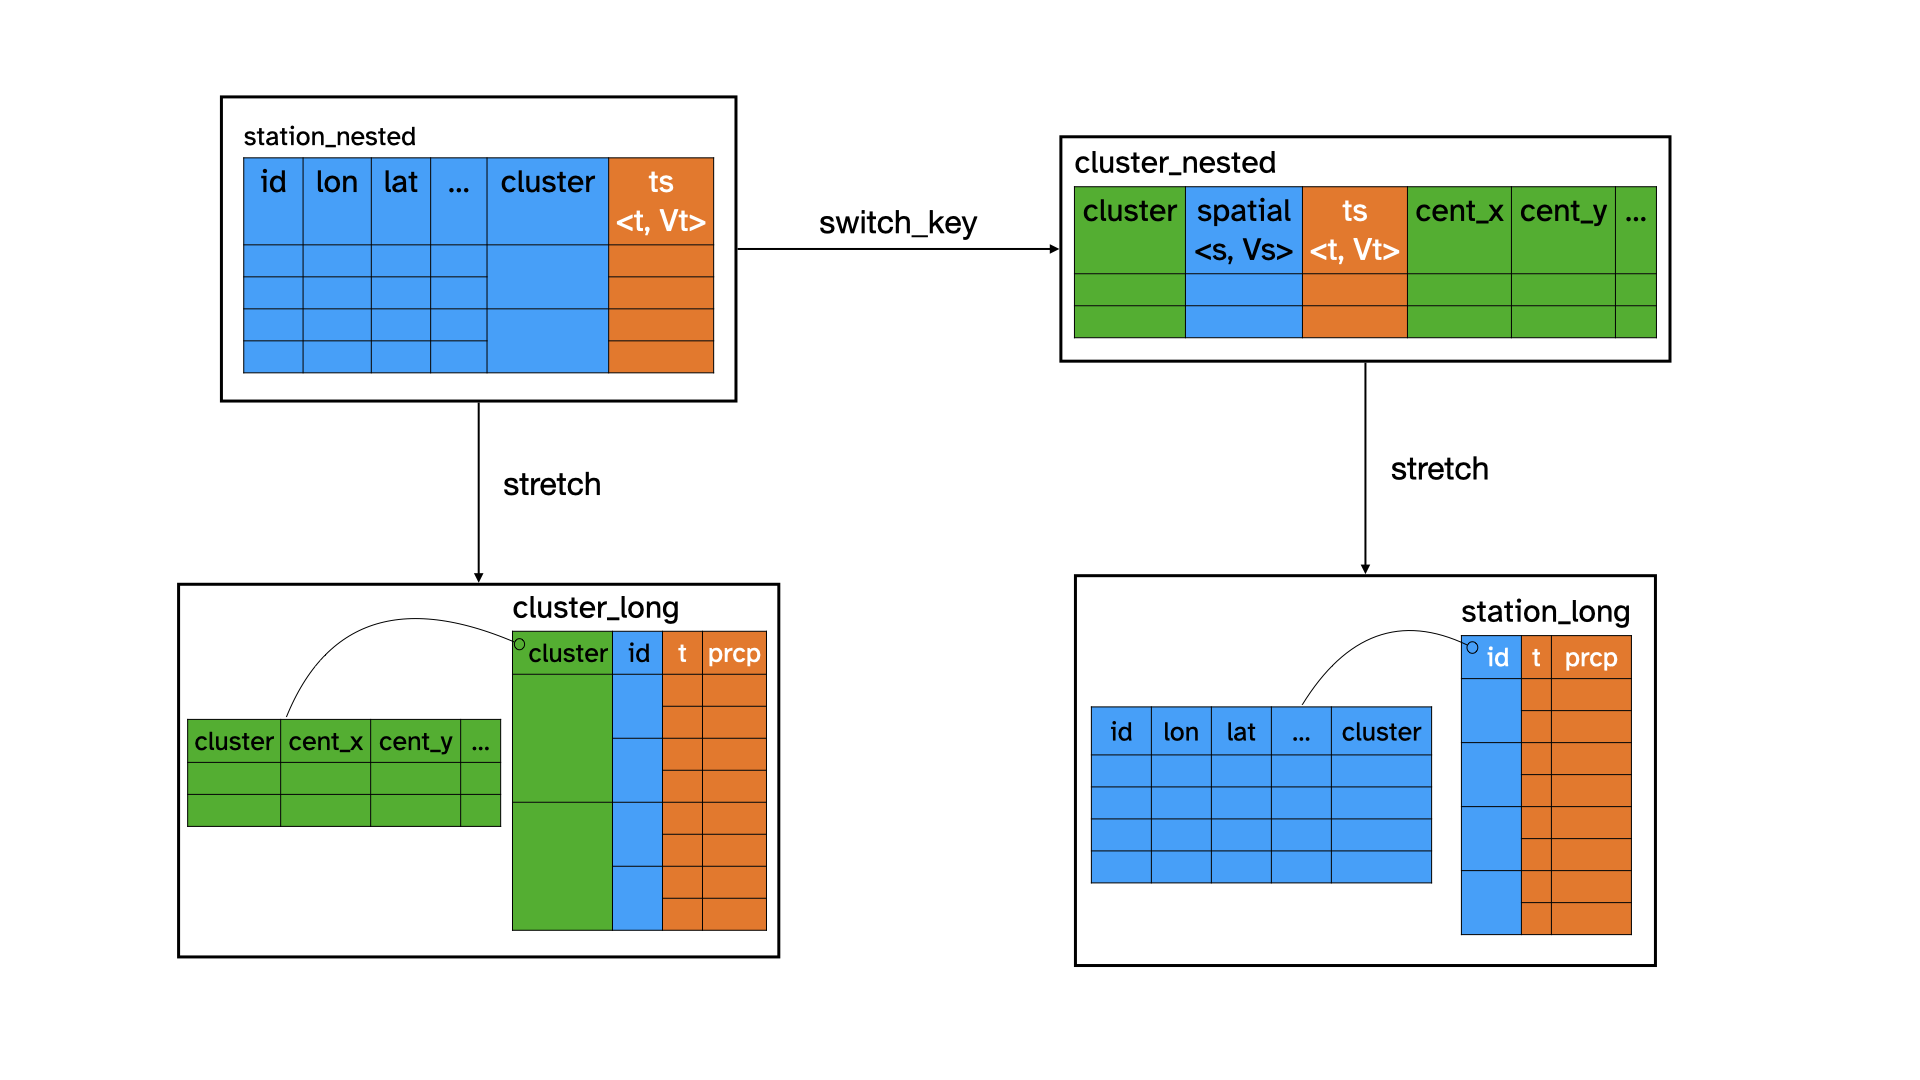
\includegraphics[width=1\linewidth,height=0.4\textheight]{/Users/sherryzhang/Documents/research/paper-cubble/figures/diagram-keynotes/diagram-keynotes.003} 

}

\caption{An illustration of the original and cluster level cubble in the nested form long form for hierarchical structure data. \code{switch\_key()} changes the station level cubble into a cluster level cubble and both can be stretched into the long form.}\label{fig:illu-hier}
\end{figure}

\hypertarget{matching}{%
\subsection{Data fusion and matching}\label{matching}}

One task that may interest analysts in spatio-temporal data is to find how similar time series, from nearby sites, are. This problem can be seen as a matching problem (\protect\hyperlink{ref-stuart2010matching}{Stuart 2010}; \protect\hyperlink{ref-mcintosh2018using}{McIntosh et al. 2018}) that pairs up similar time series in nearby locations or a data fusing exercise that merges data collected from different sources (\protect\hyperlink{ref-cocchi2019data}{Cocchi 2019}). \code{match_sites()} in \pkg{cubble} provides a simple algorithm for this task. The algorithm first matches the two data sources spatially by computing the pairwise distance on latitude and longitude. After that, pairs that pass the spatial matching are then matched temporally by computing the number of matched peaks within a fixed length moving window. Figure \ref{fig:illu-matching} illustrates this temporal matching in more detail. Given two series \code{A} and \code{a}, three peaks have been identified in each series. An interval, with default length of five, is constructed for each peak in series \code{A}, while the peaks in series \code{a} are tested against whether they fall into any of the intervals. In this illustration, there are two matches for these two series. Several arguments are available in \code{match_sites()} to fine-tune the matching:

\begin{figure}
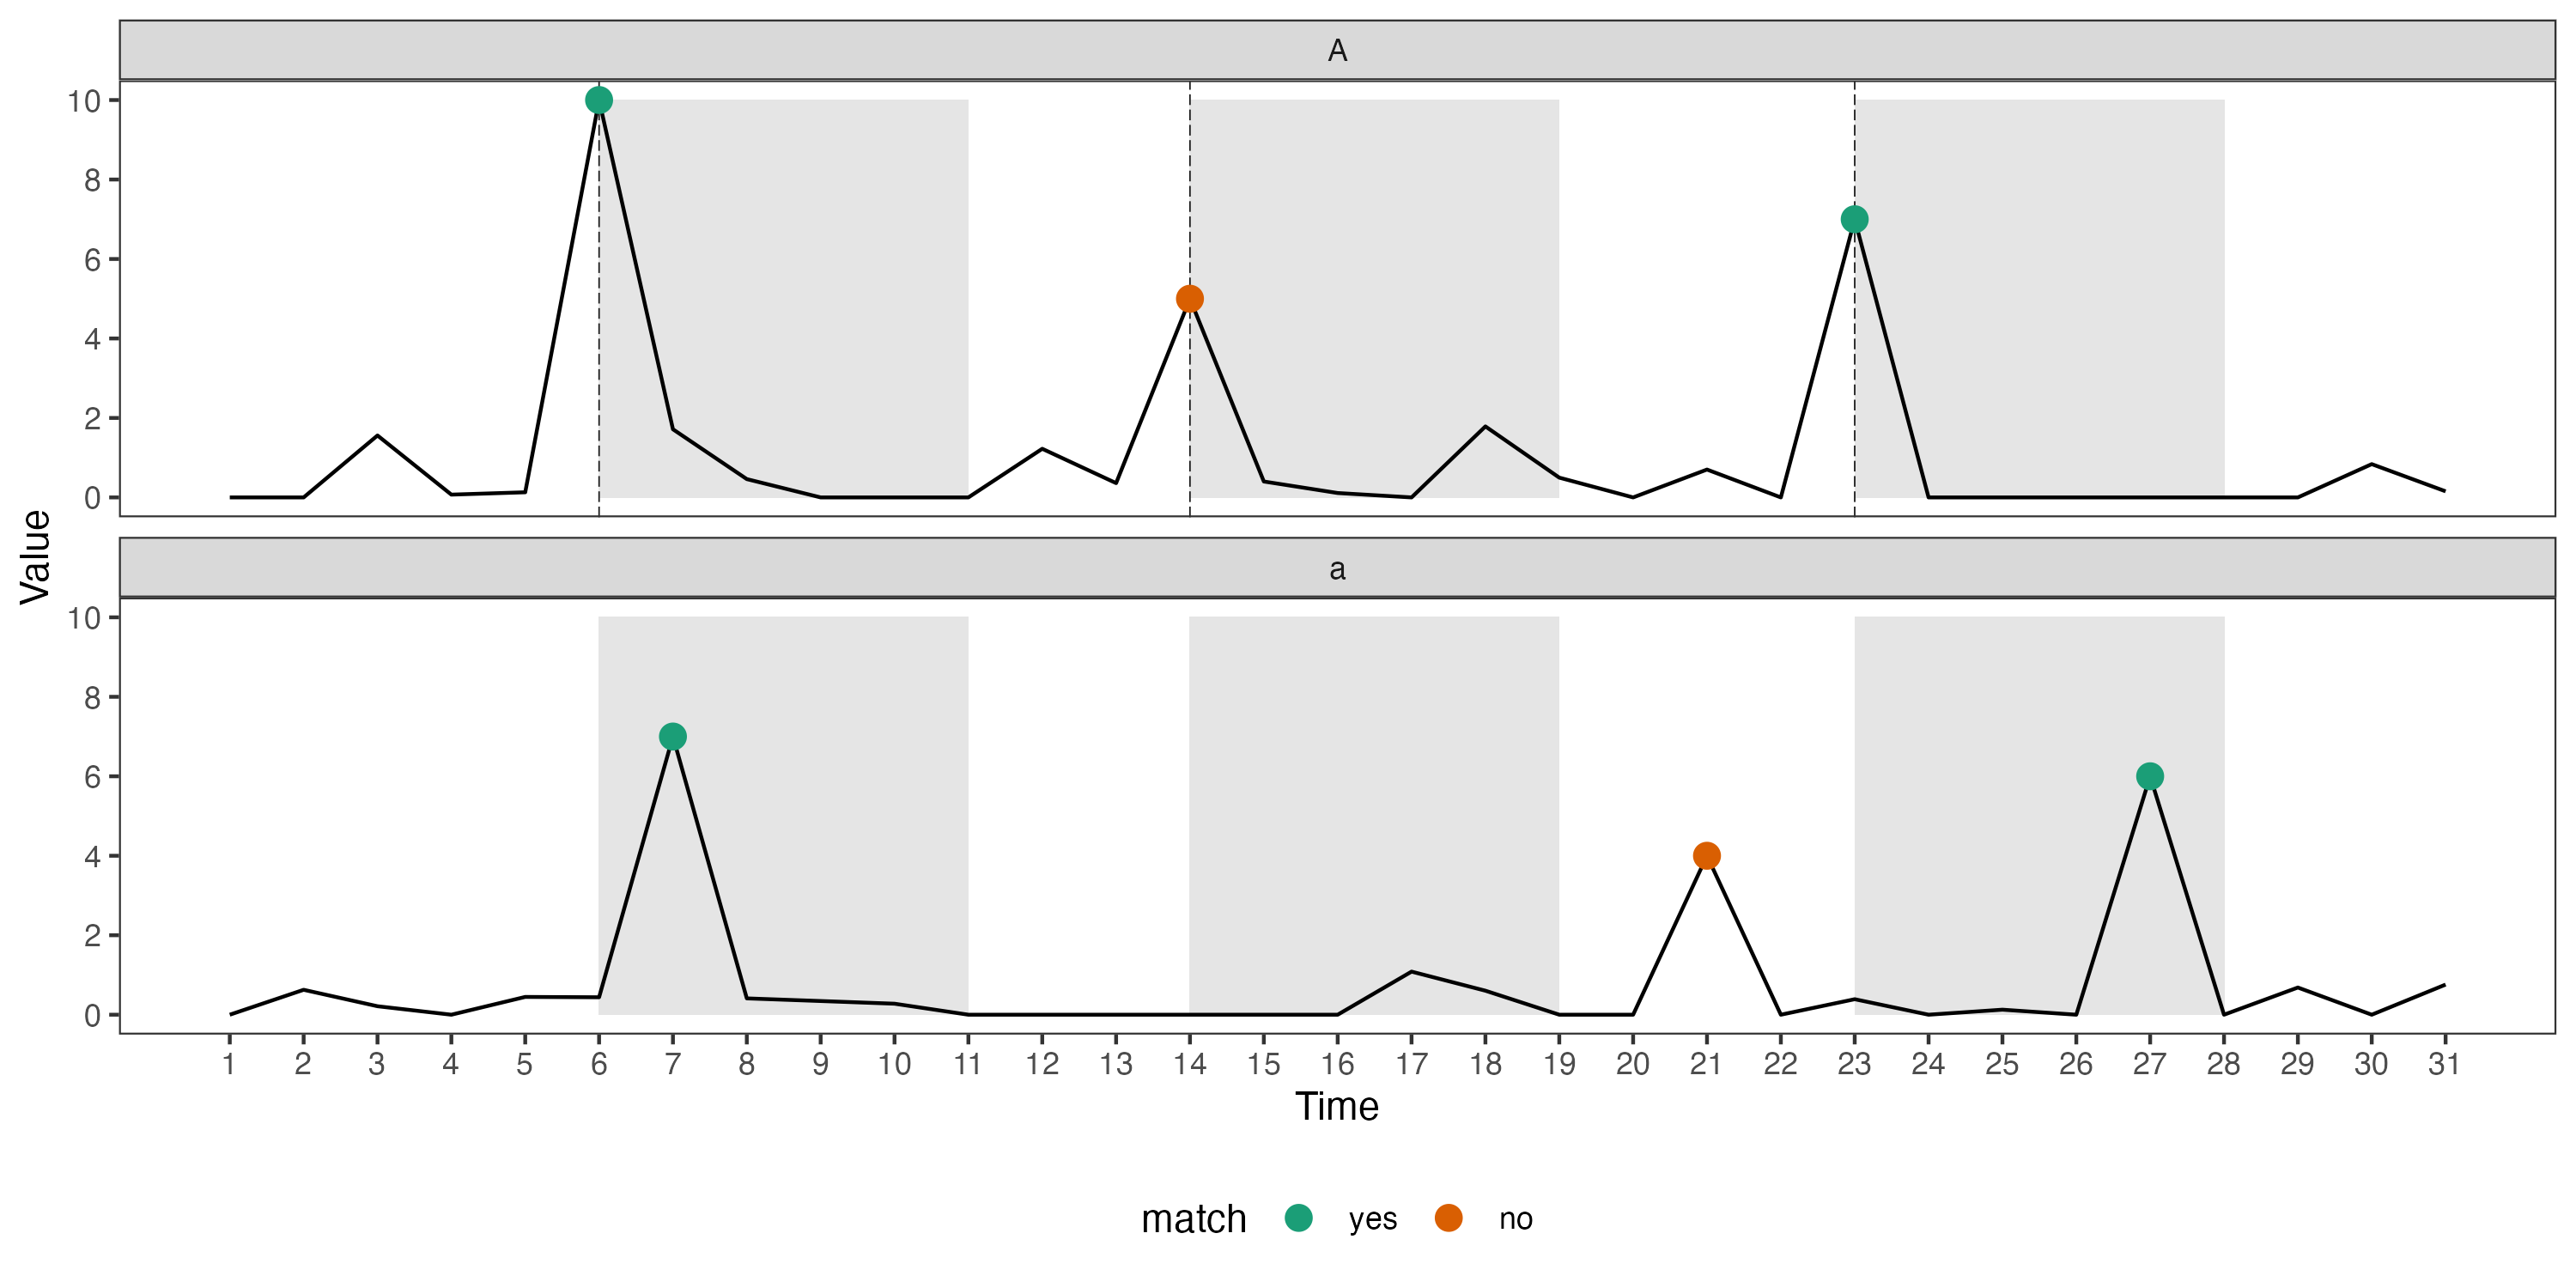
\includegraphics[width=1\linewidth]{/Users/sherryzhang/Documents/research/paper-cubble/figures/illu-matching} \caption{An illustration of temporal matching in cubble. Three highest peaks are identified in each series and intervals are constructed on series \code{A}. Two peaks in series \code{a} fall into the intervals and hence the two series are considered to have two matches.}\label{fig:illu-matching}
\end{figure}

\begin{itemize}
\tightlist
\item
  \code{spatial_n_keep}: the number of spatial match for each site to keep
\item
  \code{spatial_dist_max}: the maximum distance allowed for a matched pair
\item
  \code{temporal_n_highest}: the number of peaks used - 3 in the example above
\item
  \code{temporal_window}: the length of the interval - 5 in the example above
\item
  \code{temporal_min_match}: the minimum number of matched peaks for a valid matched pair
\end{itemize}

\hypertarget{interactive-graphics}{%
\subsection{Interactive graphics}\label{interactive-graphics}}

The linking structure of two forms in cubble fits naturally with the interactive graphic pipeline discussed in the literature (\protect\hyperlink{ref-buja1988elements}{Buja, Asimov, and Hurley 1988}; \protect\hyperlink{ref-buja1996interactive}{Buja, Cook, and Swayne 1996}; \protect\hyperlink{ref-sutherland2000orca}{Sutherland et al. 2000}; \protect\hyperlink{ref-xie2014reactive}{Xie, Hofmann, and Cheng 2014}; \protect\hyperlink{ref-cheng2016enabling}{Cheng, Cook, and Hofmann 2016}). Diagram \ref{fig:illu-interactive} illustrates how linking works from the map to the time series in cubble. The map and time series plot is associated with the nested or long cubble, respectively, and when a user action is captured on the map, the site will be activated in the nested cubble (left). The nested cubble will communicate to the long cubble to activate all the observations with the same \code{id} (middle). The long cubble will then highlight the activated series in the time series plot (right).

The linking is also available from the time series plot to the map. The selection(s) on the time series is through selecting the point(s) on the time series and once a point is selected, it will be activated in the long cubble. All the observations that share the same \code{id} are then activated and this includes other points in the same time series in the long cubble and the corresponding observation of site in the nested cubble. These activated observations will then be reflected in the updated plots and Diagram \ref{fig:illu-interactive-2} in the Appendix illustrates this process.

\begin{figure}

{\centering 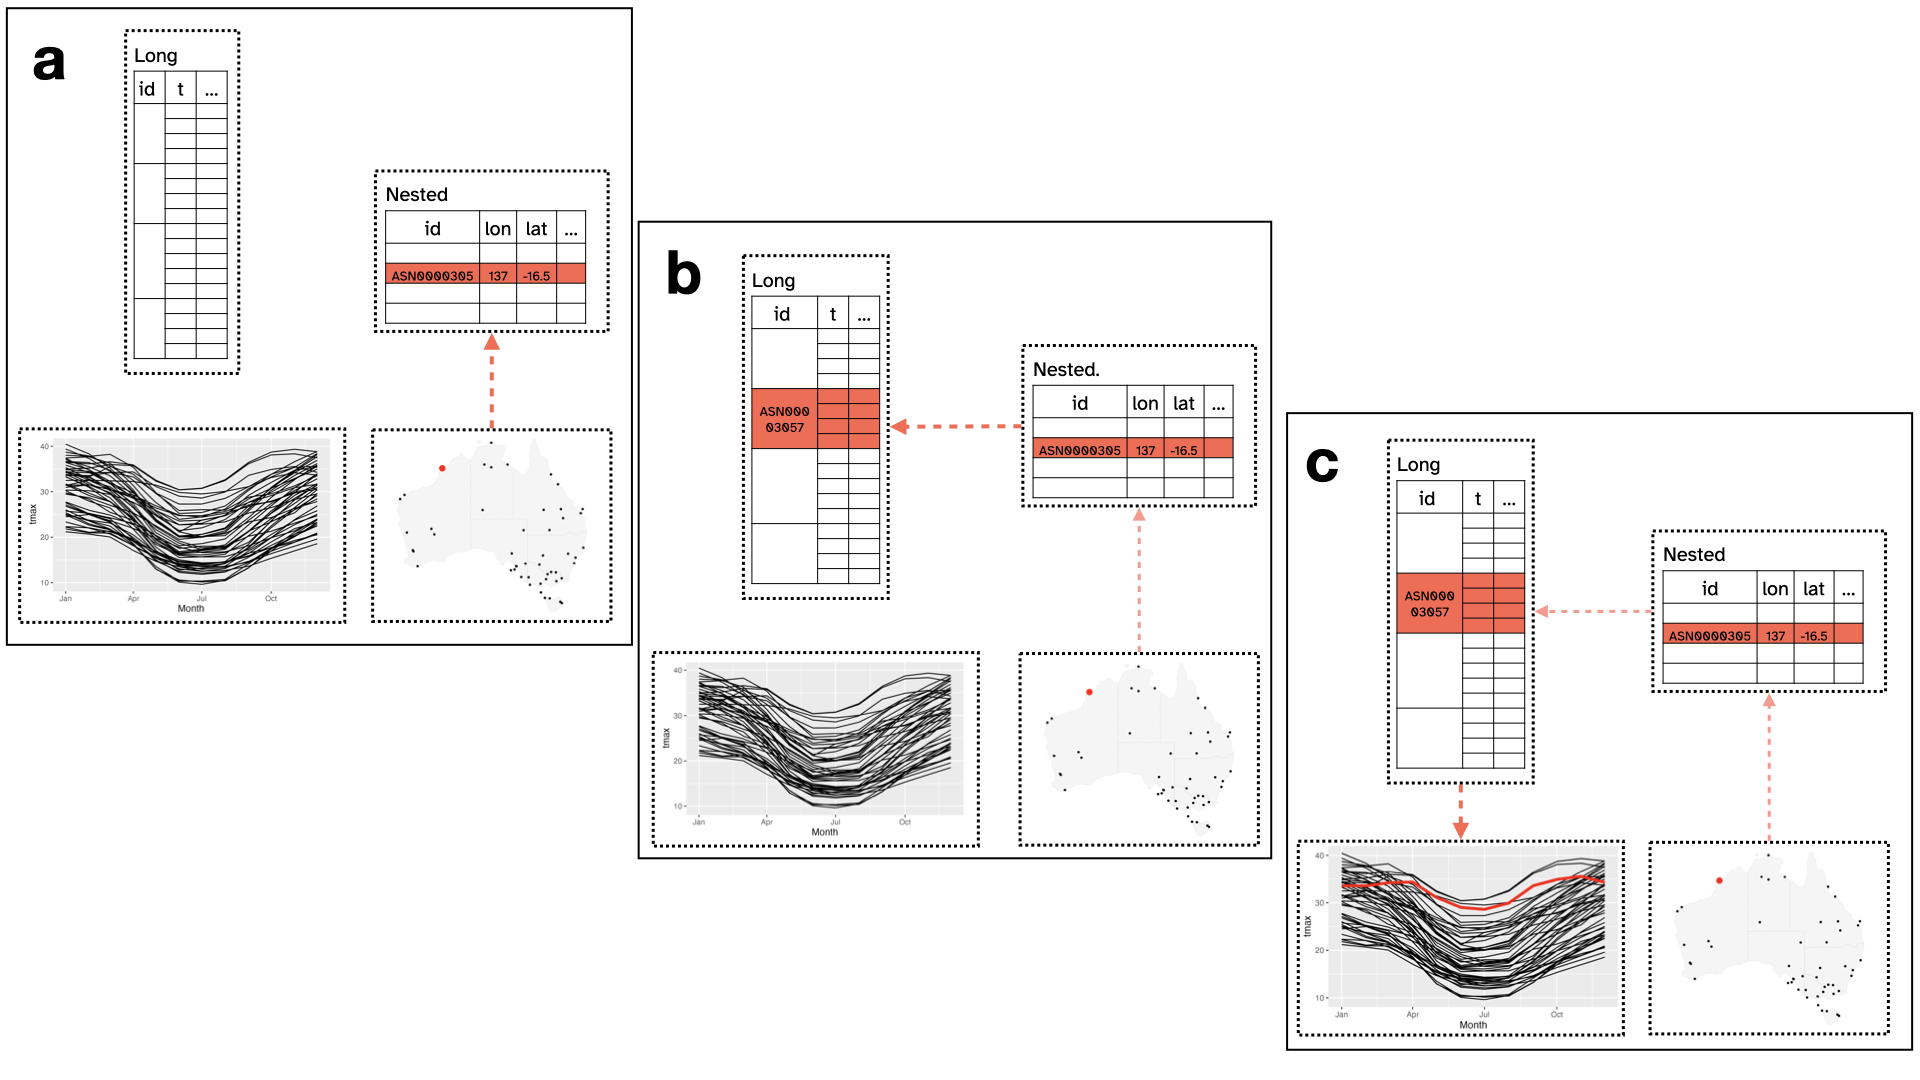
\includegraphics[width=1\linewidth,height=0.4\textheight]{/Users/sherryzhang/Documents/research/paper-cubble/figures/diagram-keynotes/diagram-keynotes.004} 

}

\caption{An illustration of the data model under interactive graphics with cubble. The line plot and the map is made separately with the long and nested cubble. When a station is selected on the map (left), the corresponding row in the nested cubble will be activated. This will link to all the rows with the same id in the long cubble (middle) and update the line plot (right).}\label{fig:illu-interactive}
\end{figure}

\hypertarget{st_transformation}{%
\subsection{Spatio-temporal transformations}\label{st_transformation}}

Different types of transformations can be useful to extract new information from spatio-temporal data. Glyph maps (\protect\hyperlink{ref-Wickham2012-yr}{Wickham et al. 2012}) transform the time coordinates into space coordinates to plot the time series of different locations on the map. Calendar plots (\protect\hyperlink{ref-wang2020calendar}{Wang, Cook, and Hyndman 2020}) reconstruct time into a calendar-based grid to discover weekday and weekend pattern. Projection, or linear combination, of variables summarises multivariate information into lower dimension to further digest. This section elaborates on the glyph map.

In \proglang{R}, \pkg{GGally} implements glyph maps through the \code{glyphs()} function. The function constructs a data frame with calculated position (\code{gx}, \code{gy}, \code{gid}) of each point on the time series using linear algebra (Equation 1 and 2 in Wickham et al. (\protect\hyperlink{ref-Wickham2012-yr}{2012})). The data can then be piped into \code{ggplot} to create the glyph map as:

\begin{Shaded}
\begin{Highlighting}[]
\FunctionTok{library}\NormalTok{(ggplot2)}
\NormalTok{gly }\OtherTok{\textless{}{-}} \FunctionTok{glyphs}\NormalTok{(data,}
              \AttributeTok{x\_major =}\NormalTok{ ..., }\AttributeTok{x\_minor =}\NormalTok{ ...,}
              \AttributeTok{y\_major =}\NormalTok{ ..., }\AttributeTok{y\_minor =}\NormalTok{ ..., ...)}

\FunctionTok{ggplot}\NormalTok{(gly, }\FunctionTok{aes}\NormalTok{(gx, gy, }\AttributeTok{group =}\NormalTok{ gid)) }\SpecialCharTok{+}
  \FunctionTok{geom\_path}\NormalTok{()}
\end{Highlighting}
\end{Shaded}

A reimplementation of the glyph map as a ggproto, \code{GeomGlyph}, has been made in the \pkg{cubble} package and now the glyph map can be created with \code{geom_glyph()}:

\begin{Shaded}
\begin{Highlighting}[]
\FunctionTok{ggplot}\NormalTok{(}\AttributeTok{data =}\NormalTok{ data) }\SpecialCharTok{+}
  \FunctionTok{geom\_glyph}\NormalTok{(}\FunctionTok{aes}\NormalTok{(}\AttributeTok{x\_major =}\NormalTok{ ..., }\AttributeTok{x\_minor =}\NormalTok{ ...,}
                 \AttributeTok{y\_major =}\NormalTok{ ..., }\AttributeTok{y\_minor =}\NormalTok{ ...))}
\end{Highlighting}
\end{Shaded}

Some useful controls over the glyph map are also available in the \code{geom_glyph()} implementation. Polar glyph map can be specified as a parameter \code{polar = TRUE} in the \code{geom_glyph()}, along with \code{width} and \code{height} in either absolute or relative value. Global and local scale can be controlled by the parameter \code{global_rescale} which default to \code{TRUE} for global scaling. Reference box and line can be added with separate \code{geom_glyph_box()} and \code{geom_glyph_line()}.

\hypertarget{examples}{%
\section{Examples}\label{examples}}

\hypertarget{covid}{%
\subsection{Victoria covid data}\label{covid}}

The Victoria State Government in Australia provides daily COVID information about the source, and local government area (LGA) of the recorded cases. This data can be used to visualise COVID spread when combined with map information on LGA, available from the Australian Bureau of Statistics. The first five rows these data sets are printed below:

\begin{Shaded}
\begin{Highlighting}[]
\NormalTok{covid }\SpecialCharTok{|\textgreater{}} \FunctionTok{head}\NormalTok{(}\DecValTok{5}\NormalTok{)}
\end{Highlighting}
\end{Shaded}

\begin{verbatim}
## # A tsibble: 5 x 5 [1D]
## # Key:       lga [1]
## # Groups:    lga, source [1]
##   date       lga        source                            n roll_mean
##   <date>     <chr>      <chr>                         <int>     <dbl>
## 1 2022-01-01 Alpine (S) Contact with a confirmed case     1        NA
## 2 2022-01-02 Alpine (S) Contact with a confirmed case     2        NA
## 3 2022-01-03 Alpine (S) Contact with a confirmed case     4        NA
## 4 2022-01-04 Alpine (S) Contact with a confirmed case     4        NA
## 5 2022-01-05 Alpine (S) Contact with a confirmed case     2        NA
\end{verbatim}

\begin{Shaded}
\begin{Highlighting}[]
\NormalTok{lga }\SpecialCharTok{|\textgreater{}} \FunctionTok{head}\NormalTok{(}\DecValTok{5}\NormalTok{)}
\end{Highlighting}
\end{Shaded}

\begin{verbatim}
## Simple feature collection with 5 features and 7 fields
## Geometry type: MULTIPOLYGON
## Dimension:     XY
## Bounding box:  xmin: 142.3535 ymin: -38.67876 xmax: 147.3909 ymax: -36.39269
## Geodetic CRS:  WGS 84
##     lga_code_2018            lga state_code_2016 state_name_2016 areasqkm_2018
## 132         20110     Alpine (S)               2        Victoria     4788.1568
## 133         20260    Ararat (RC)               2        Victoria     4211.1171
## 134         20570   Ballarat (C)               2        Victoria      739.0321
## 135         20660    Banyule (C)               2        Victoria       62.5402
## 136         20740 Bass Coast (S)               2        Victoria      865.8095
##     cent_long  cent_lat                       geometry
## 132  146.9742 -36.85357 MULTIPOLYGON (((146.7258 -3...
## 133  142.8432 -37.47271 MULTIPOLYGON (((143.1807 -3...
## 134  143.7815 -37.49286 MULTIPOLYGON (((143.6622 -3...
## 135  145.0851 -37.73043 MULTIPOLYGON (((145.1357 -3...
## 136  145.5581 -38.50730 MULTIPOLYGON (((145.5207 -3...
\end{verbatim}

A \code{cubble} object can be created from separate spatial and temporal tables in a list, with other arguments (\code{key}, \code{index}, and \code{coords}) introduced in Section \ref{create}. \code{as_cubble()} will automatically check the matching of sites in both tables and emit a warning if a location has missing spatial or temporal information.

\begin{Shaded}
\begin{Highlighting}[]
\NormalTok{cb }\OtherTok{\textless{}{-}} \FunctionTok{as\_cubble}\NormalTok{(}\FunctionTok{list}\NormalTok{(}\AttributeTok{spatial =}\NormalTok{ lga, }\AttributeTok{temporal =}\NormalTok{ covid),}
                \AttributeTok{key =}\NormalTok{ lga, }\AttributeTok{index =}\NormalTok{ date, }\AttributeTok{coords =} \FunctionTok{c}\NormalTok{(cent\_long, cent\_lat))}
\end{Highlighting}
\end{Shaded}

\begin{verbatim}
## ! Some sites in the temporal table don't have corresponding spatial information
\end{verbatim}

\begin{verbatim}
## ! Some sites in the spatial table don't have corresponding temporal information
\end{verbatim}

\begin{verbatim}
## ! Use argument `output = "unmatch"` to check on the unmatched key
\end{verbatim}

Here, some locations have been detected with this issue and you can use \code{output = "unmatch"} to check on these locations:

\begin{Shaded}
\begin{Highlighting}[]
\NormalTok{pair }\OtherTok{\textless{}{-}} \FunctionTok{as\_cubble}\NormalTok{(}\FunctionTok{list}\NormalTok{(}\AttributeTok{spatial =}\NormalTok{ lga, }\AttributeTok{temporal =}\NormalTok{ covid),}
                  \AttributeTok{key =}\NormalTok{ lga, }\AttributeTok{index =}\NormalTok{ date, }\AttributeTok{coords =} \FunctionTok{c}\NormalTok{(cent\_long, cent\_lat),}
                  \AttributeTok{output =} \StringTok{"unmatch"}\NormalTok{)}

\NormalTok{pair}
\end{Highlighting}
\end{Shaded}

\begin{verbatim}
## $paired
## # A tibble: 2 x 2
##   spatial             temporal    
##   <chr>               <chr>       
## 1 Kingston (C) (Vic.) Kingston (C)
## 2 Latrobe (C) (Vic.)  Latrobe (C) 
## 
## $others
## $others$temporal
## [1] "Interstate" "Overseas"   "Unknown"   
## 
## $others$spatial
## [1] "No usual address (Vic.)"               
## [2] "Migratory - Offshore - Shipping (Vic.)"
\end{verbatim}

\pkg{cubble} will attempt to pair the unmatched sites as well as those that cannot be paired. These can be helpful to clean up the data before creating the cubble again:

\begin{Shaded}
\begin{Highlighting}[]
\NormalTok{lga }\OtherTok{\textless{}{-}}\NormalTok{ lga }\SpecialCharTok{\%\textgreater{}\%}
  \FunctionTok{mutate}\NormalTok{(}\AttributeTok{lga =} \FunctionTok{ifelse}\NormalTok{(lga }\SpecialCharTok{==} \StringTok{"Kingston (C) (Vic.)"}\NormalTok{, }\StringTok{"Kingston (C)"}\NormalTok{, lga),}
         \AttributeTok{lga =} \FunctionTok{ifelse}\NormalTok{(lga }\SpecialCharTok{==} \StringTok{"Latrobe (C) (Vic.)"}\NormalTok{, }\StringTok{"Latrobe (C)"}\NormalTok{, lga)) }\SpecialCharTok{\%\textgreater{}\%}
  \FunctionTok{filter}\NormalTok{(}\SpecialCharTok{!}\NormalTok{lga }\SpecialCharTok{\%in\%}\NormalTok{ pair}\SpecialCharTok{$}\NormalTok{others}\SpecialCharTok{$}\NormalTok{spatial)}

\NormalTok{covid }\OtherTok{\textless{}{-}}\NormalTok{ covid }\SpecialCharTok{\%\textgreater{}\%} \FunctionTok{filter}\NormalTok{(}\SpecialCharTok{!}\NormalTok{lga }\SpecialCharTok{\%in\%}\NormalTok{ pair}\SpecialCharTok{$}\NormalTok{others}\SpecialCharTok{$}\NormalTok{temporal)}

\NormalTok{cb }\OtherTok{\textless{}{-}} \FunctionTok{as\_cubble}\NormalTok{(}\AttributeTok{data =} \FunctionTok{list}\NormalTok{(}\AttributeTok{spatial =}\NormalTok{ lga, }\AttributeTok{temporal =}\NormalTok{ covid),}
                \AttributeTok{key =}\NormalTok{ lga, }\AttributeTok{index =}\NormalTok{ date, }\AttributeTok{coords =} \FunctionTok{c}\NormalTok{(cent\_long, cent\_lat))}
\end{Highlighting}
\end{Shaded}

\hypertarget{australian-historical-maximum-temperature}{%
\subsection{Australian historical maximum temperature}\label{australian-historical-maximum-temperature}}

The Global Historical Climatology Network (GHCN) provides daily climate measures from stations across the world. The dataset \code{weatherdata::historical_tmax} extracts the maximum temperature for 236 Australian stations from the GHCN starting from year 1969. \code{weatherdata::historical_tmax} is already in a cubble, with \code{id} as the key, \code{date} as the index, and \code{c(longitude, latitude)} as the coordinates. This example compares the maximum temperature in two periods: 1971-1975 and 2016-2020 for stations in Victoria and New South Wales.

Stations in the two states can be subsetted by the station number: the Australian GHCN station numbers start with ``ASN00'' and are followed by the \href{http://www.bom.gov.au/climate/cdo/about/site-num.shtml}{Bureau of Meteorology (BOM) station number}. The second and third digits of the BOM station number (7th and 8th in the GHCN number) define the state of the station; the range 46-75 corresponds to New South Wales stations and the range 76-90 corresponds to Victorian stations. Filtering Victoria and New South Wales stations is a spatial operation and hence uses the nested form:

\begin{Shaded}
\begin{Highlighting}[]
\NormalTok{tmax }\OtherTok{\textless{}{-}}\NormalTok{ weatherdata}\SpecialCharTok{::}\NormalTok{historical\_tmax }\SpecialCharTok{|\textgreater{}}
  \FunctionTok{filter}\NormalTok{(}\FunctionTok{between}\NormalTok{(stringr}\SpecialCharTok{::}\FunctionTok{str\_sub}\NormalTok{(id, }\DecValTok{7}\NormalTok{, }\DecValTok{8}\NormalTok{), }\DecValTok{46}\NormalTok{, }\DecValTok{90}\NormalTok{))}
\end{Highlighting}
\end{Shaded}

Filtering for the time periods 1971-1975 and 2016-2020 is a time operation and the nested cubble needs to be switched to the long cubble form by \code{stretch()}:

\begin{Shaded}
\begin{Highlighting}[]
\NormalTok{tmax }\OtherTok{\textless{}{-}}\NormalTok{ tmax }\SpecialCharTok{|\textgreater{}}
  \FunctionTok{face\_temporal}\NormalTok{() }\SpecialCharTok{|\textgreater{}}
  \FunctionTok{filter}\NormalTok{(lubridate}\SpecialCharTok{::}\FunctionTok{year}\NormalTok{(date) }\SpecialCharTok{\%in\%} \FunctionTok{c}\NormalTok{(}\DecValTok{1971}\SpecialCharTok{:}\DecValTok{1975}\NormalTok{, }\DecValTok{2016}\SpecialCharTok{:}\DecValTok{2020}\NormalTok{))}
\end{Highlighting}
\end{Shaded}

A monthly average is used for both periods to smooth the maximum temperature, which is another time operation:

\begin{Shaded}
\begin{Highlighting}[]
\NormalTok{tmax }\OtherTok{\textless{}{-}}\NormalTok{ tmax }\SpecialCharTok{|\textgreater{}}
  \FunctionTok{group\_by}\NormalTok{(}\AttributeTok{month =}\NormalTok{ lubridate}\SpecialCharTok{::}\FunctionTok{month}\NormalTok{(date),}
         \AttributeTok{group =} \FunctionTok{as.factor}\NormalTok{(}\FunctionTok{ifelse}\NormalTok{(lubridate}\SpecialCharTok{::}\FunctionTok{year}\NormalTok{(date) }\SpecialCharTok{\textgreater{}} \DecValTok{2015}\NormalTok{,}
                                  \StringTok{"2016 \textasciitilde{} 2020"}\NormalTok{, }\StringTok{"1971 \textasciitilde{} 1975"}\NormalTok{))) }\SpecialCharTok{|\textgreater{}}
  \FunctionTok{summarise}\NormalTok{(}\AttributeTok{tmax =} \FunctionTok{mean}\NormalTok{(tmax, }\AttributeTok{na.rm =} \ConstantTok{TRUE}\NormalTok{))}
\end{Highlighting}
\end{Shaded}

A few stations do not have records during the time period 1971-1975 and further investigation shows that while the first and last year of each series is recorded, the missing years in this period are not reported. These stations are filtered out by examining whether the summarised time series has 24 months. The long cubble needs to be switched to the nested form for this spatial operation using \code{face_spatial()}:

\begin{Shaded}
\begin{Highlighting}[]
\NormalTok{tmax }\OtherTok{\textless{}{-}}\NormalTok{ tmax }\SpecialCharTok{|\textgreater{}} \FunctionTok{face\_spatial}\NormalTok{() }\SpecialCharTok{|\textgreater{}} \FunctionTok{filter}\NormalTok{(}\FunctionTok{nrow}\NormalTok{(ts) }\SpecialCharTok{==} \DecValTok{24}\NormalTok{)}
\end{Highlighting}
\end{Shaded}

Lastly, to create a glyph map, both the major (\code{longitude}, \code{latitude}) and minor (\code{month}, \code{tmax}) coordinates need to be in the same table. Spatial variables can be moved to the long form with \code{unfold()}:

\begin{Shaded}
\begin{Highlighting}[]
\NormalTok{tmax }\OtherTok{\textless{}{-}}\NormalTok{ tmax }\SpecialCharTok{|\textgreater{}} \FunctionTok{face\_temporal}\NormalTok{() }\SpecialCharTok{|\textgreater{}} \FunctionTok{unfold}\NormalTok{(latitude, longitude)}
\end{Highlighting}
\end{Shaded}

\code{tmax} can then be supplied to \code{geom_glyph()} for the glyph map in Figure \ref{fig:basic-manip} with a station inset on the top left corner:

\begin{Shaded}
\begin{Highlighting}[]
\NormalTok{nsw\_vic }\OtherTok{\textless{}{-}}\NormalTok{ ozmaps}\SpecialCharTok{::}\NormalTok{abs\_ste }\SpecialCharTok{|\textgreater{}}
  \FunctionTok{filter}\NormalTok{(NAME }\SpecialCharTok{\%in\%} \FunctionTok{c}\NormalTok{(}\StringTok{"Victoria"}\NormalTok{, }\StringTok{"New South Wales"}\NormalTok{))}

\FunctionTok{ggplot}\NormalTok{() }\SpecialCharTok{+}
  \FunctionTok{geom\_sf}\NormalTok{(}\AttributeTok{data =}\NormalTok{ nsw\_vic,}
          \AttributeTok{fill =} \StringTok{"transparent"}\NormalTok{, }\AttributeTok{color =} \StringTok{"grey"}\NormalTok{, }\AttributeTok{linetype =} \StringTok{"dotted"}\NormalTok{) }\SpecialCharTok{+}
  \FunctionTok{geom\_glyph}\NormalTok{(}\AttributeTok{data =}\NormalTok{ tmax,}
             \FunctionTok{aes}\NormalTok{(}\AttributeTok{x\_major =}\NormalTok{ longitude, }\AttributeTok{x\_minor =}\NormalTok{ month,}
                 \AttributeTok{y\_major =}\NormalTok{ latitude, }\AttributeTok{y\_minor =}\NormalTok{ tmax,}
                 \AttributeTok{group =} \FunctionTok{interaction}\NormalTok{(id, group), }\AttributeTok{color =}\NormalTok{ group),}
             \AttributeTok{width =} \DecValTok{1}\NormalTok{, }\AttributeTok{height =} \FloatTok{0.5}\NormalTok{) }\SpecialCharTok{+}
\NormalTok{  ...}
\end{Highlighting}
\end{Shaded}

\begin{figure}
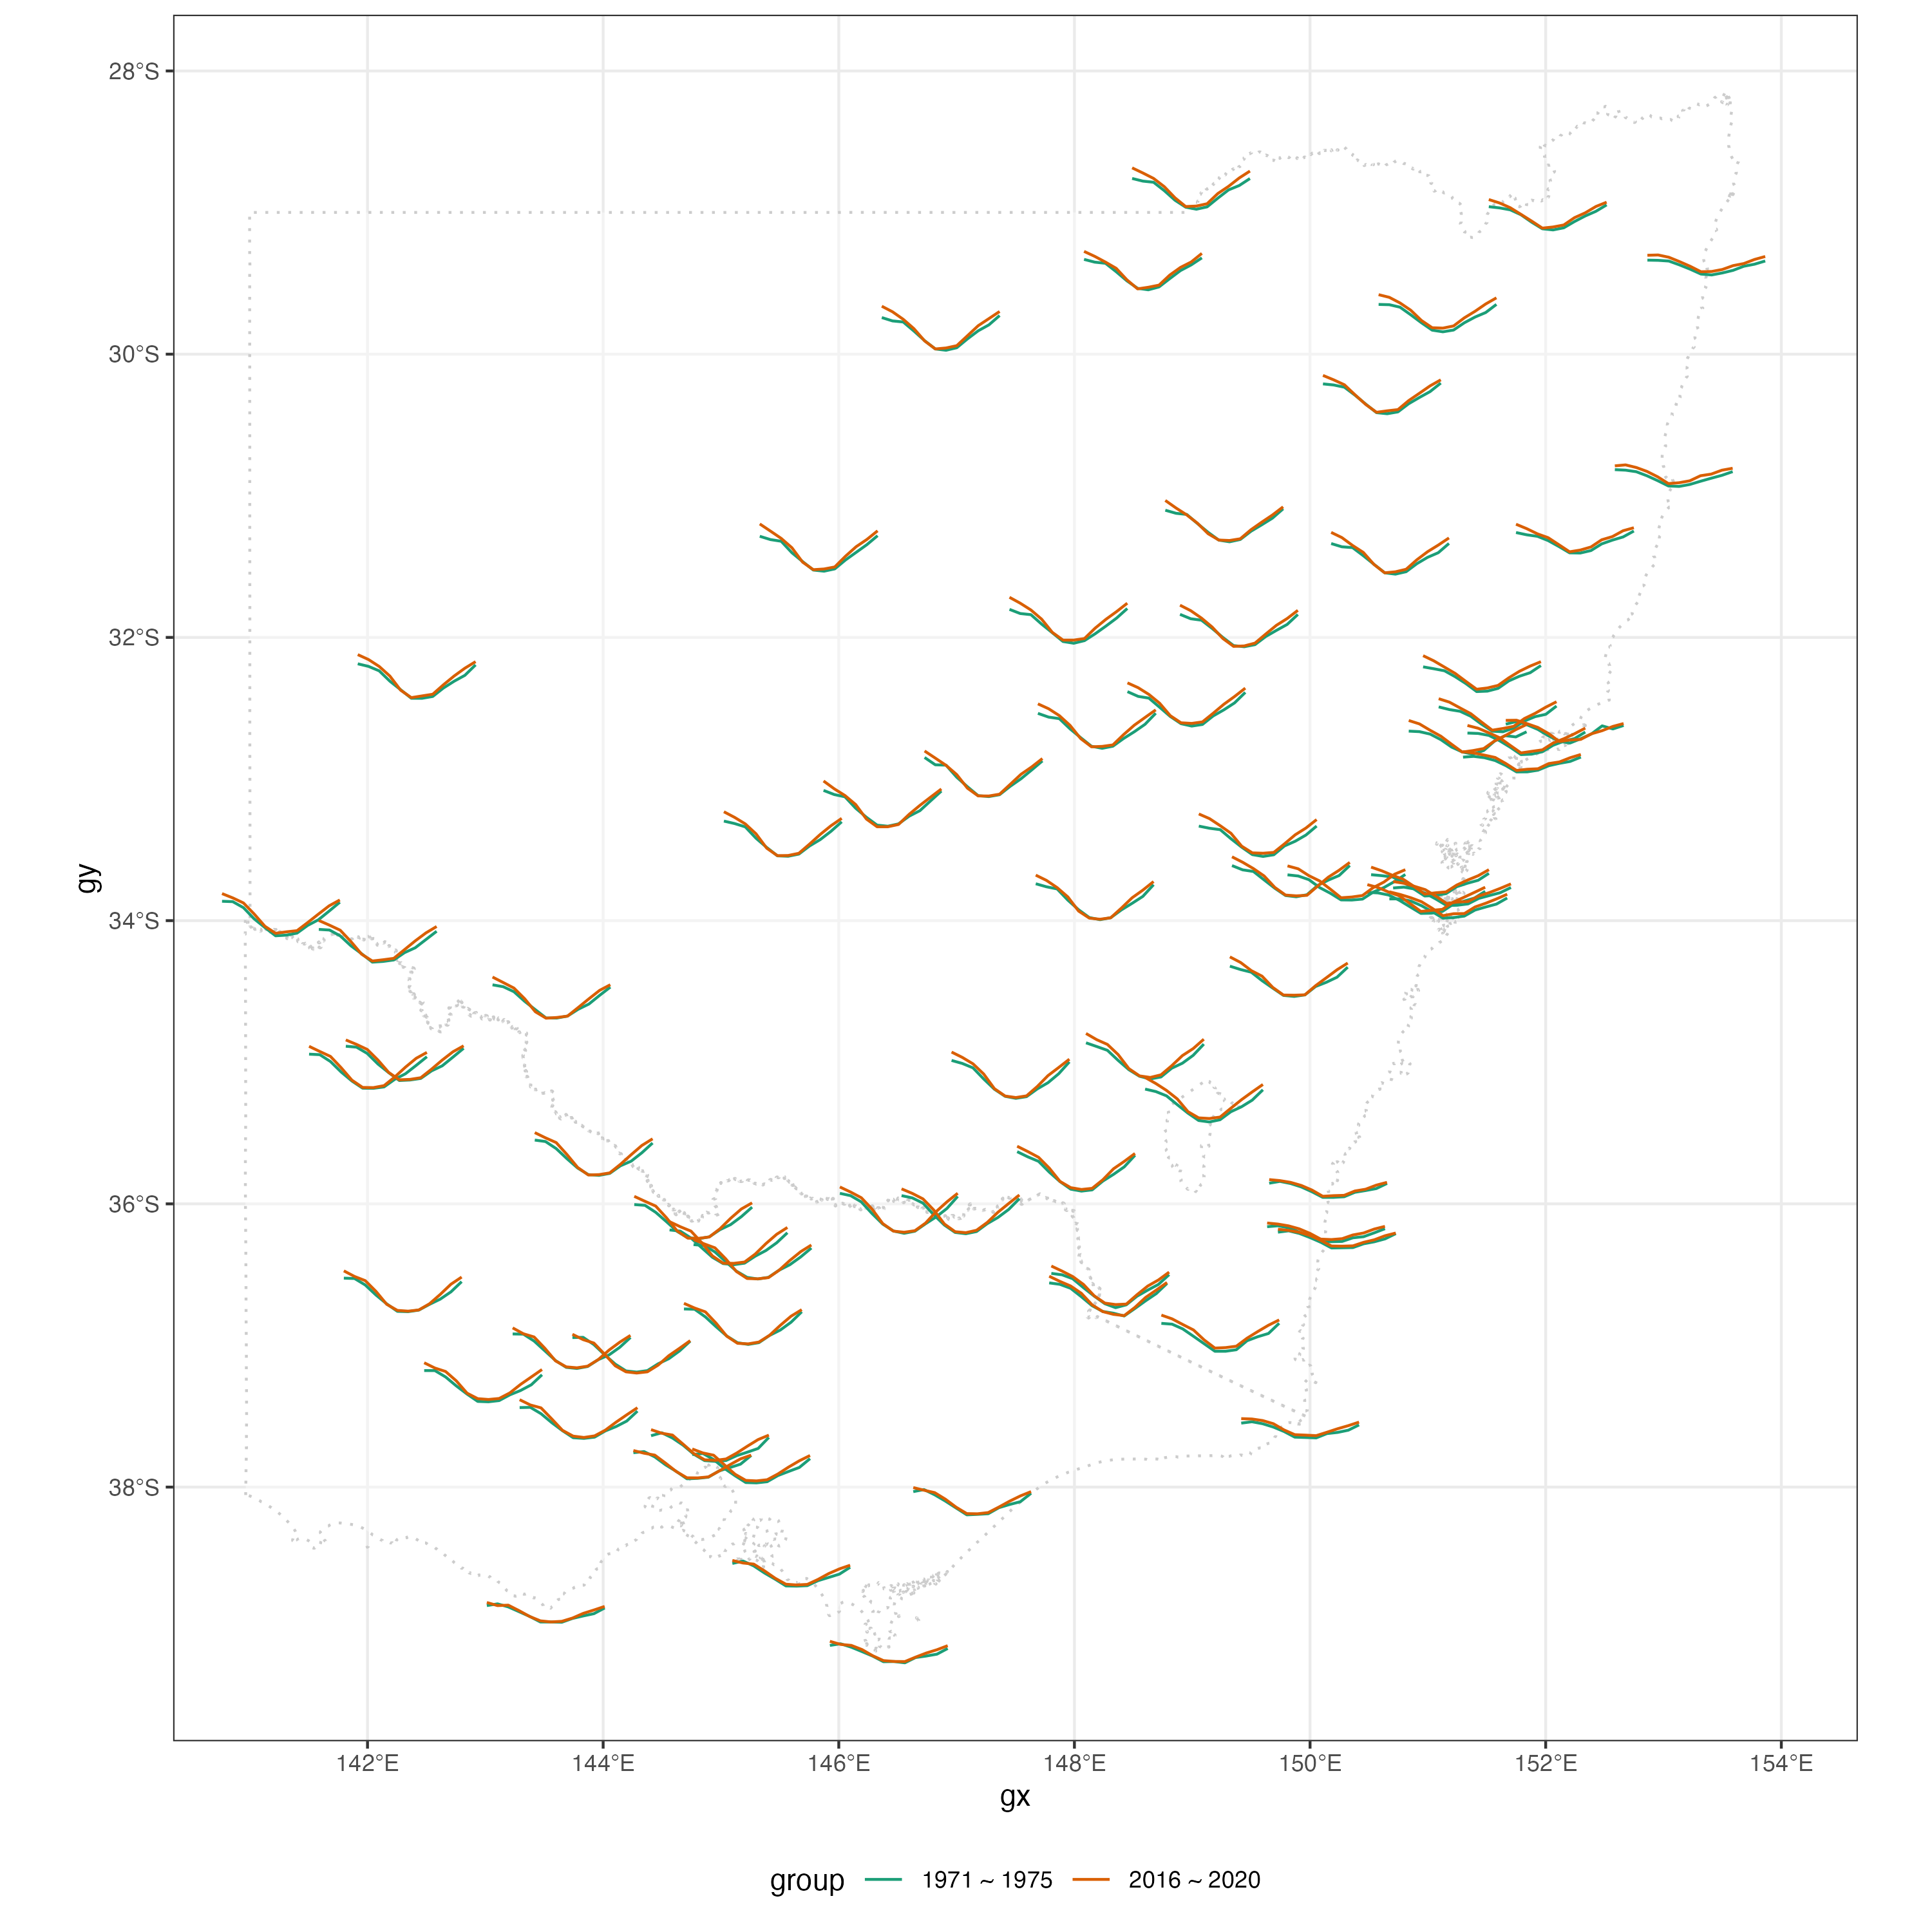
\includegraphics[width=1\linewidth,height=0.7\textheight]{/Users/sherryzhang/Documents/research/paper-cubble/figures/basic-manip} \caption{A glyph map of the average maximum temperature by month of Victoria and New South Wales weather stations in Australia. On the top left corner is an insetted plot of station Cobar highlighted in the black box.}\label{fig:basic-manip}
\end{figure}

\hypertarget{australia-precipitation-pattern-in-2020}{%
\subsection{Australia precipitation pattern in 2020}\label{australia-precipitation-pattern-in-2020}}

In the previous example, there has already been some overlapping of the glyphs for a few stations near (151E, 34S) and (152E, 33S), which is a problem when mapping more stations at the national level. Aggregation can be helpful in grouping series into clusters before visualising the clusters with a glyph map. This example shows how to organise data at both levels with \code{switch_key()}.

\code{weatherdata::climate_full}, also extracted from the GHCN, records daily precipitation and maximum/minimum temperature for 639 stations in Australia from 2016 to 2020. A simple \(k\)-means algorithm based on the distance matrix is used to create 20 clusters. The dataset \code{station_nested} is a nested cubble with a cluster column indicating the group to which each station belongs. More advanced clustering algorithms can be used for other applications, as long as there is a mapping from each station to a cluster.

\begin{Shaded}
\begin{Highlighting}[]
\NormalTok{station\_nested }\OtherTok{\textless{}{-}}\NormalTok{ weatherdata}\SpecialCharTok{::}\NormalTok{climate\_full }\SpecialCharTok{|\textgreater{}}
  \FunctionTok{mutate}\NormalTok{(}\AttributeTok{cluster =}\NormalTok{ ...)}
\end{Highlighting}
\end{Shaded}

To create a group-level cubble, use \code{switch_key()} with the new key variable, \code{cluster}:

\begin{Shaded}
\begin{Highlighting}[]
\NormalTok{cluster\_nested }\OtherTok{\textless{}{-}}\NormalTok{ station\_nested }\SpecialCharTok{|\textgreater{}} \FunctionTok{switch\_key}\NormalTok{(cluster)}
\end{Highlighting}
\end{Shaded}

With the group-level cubble, \code{get_centroid()} is useful to compute the centroid of each cluster, which will be used as the major axis for the glyph map later:

\begin{Shaded}
\begin{Highlighting}[]
\NormalTok{cluster\_nested }\OtherTok{\textless{}{-}}\NormalTok{ cluster\_nested }\SpecialCharTok{|\textgreater{}} \FunctionTok{get\_centroid}\NormalTok{()}
\end{Highlighting}
\end{Shaded}

Long form cubble at both levels can be accessed through stretching the nested form and with access to both station and cluster-level cubbles, various plots can be made to understand the cluster. Figure \ref{fig:basic-agg} shows two example plots that can be made with this data. Subplot A is a glyph map made with the cluster level cubble in the long form and subplot B inspects the station membership of each cluster using the station level cubble in the nested form.

\begin{figure}
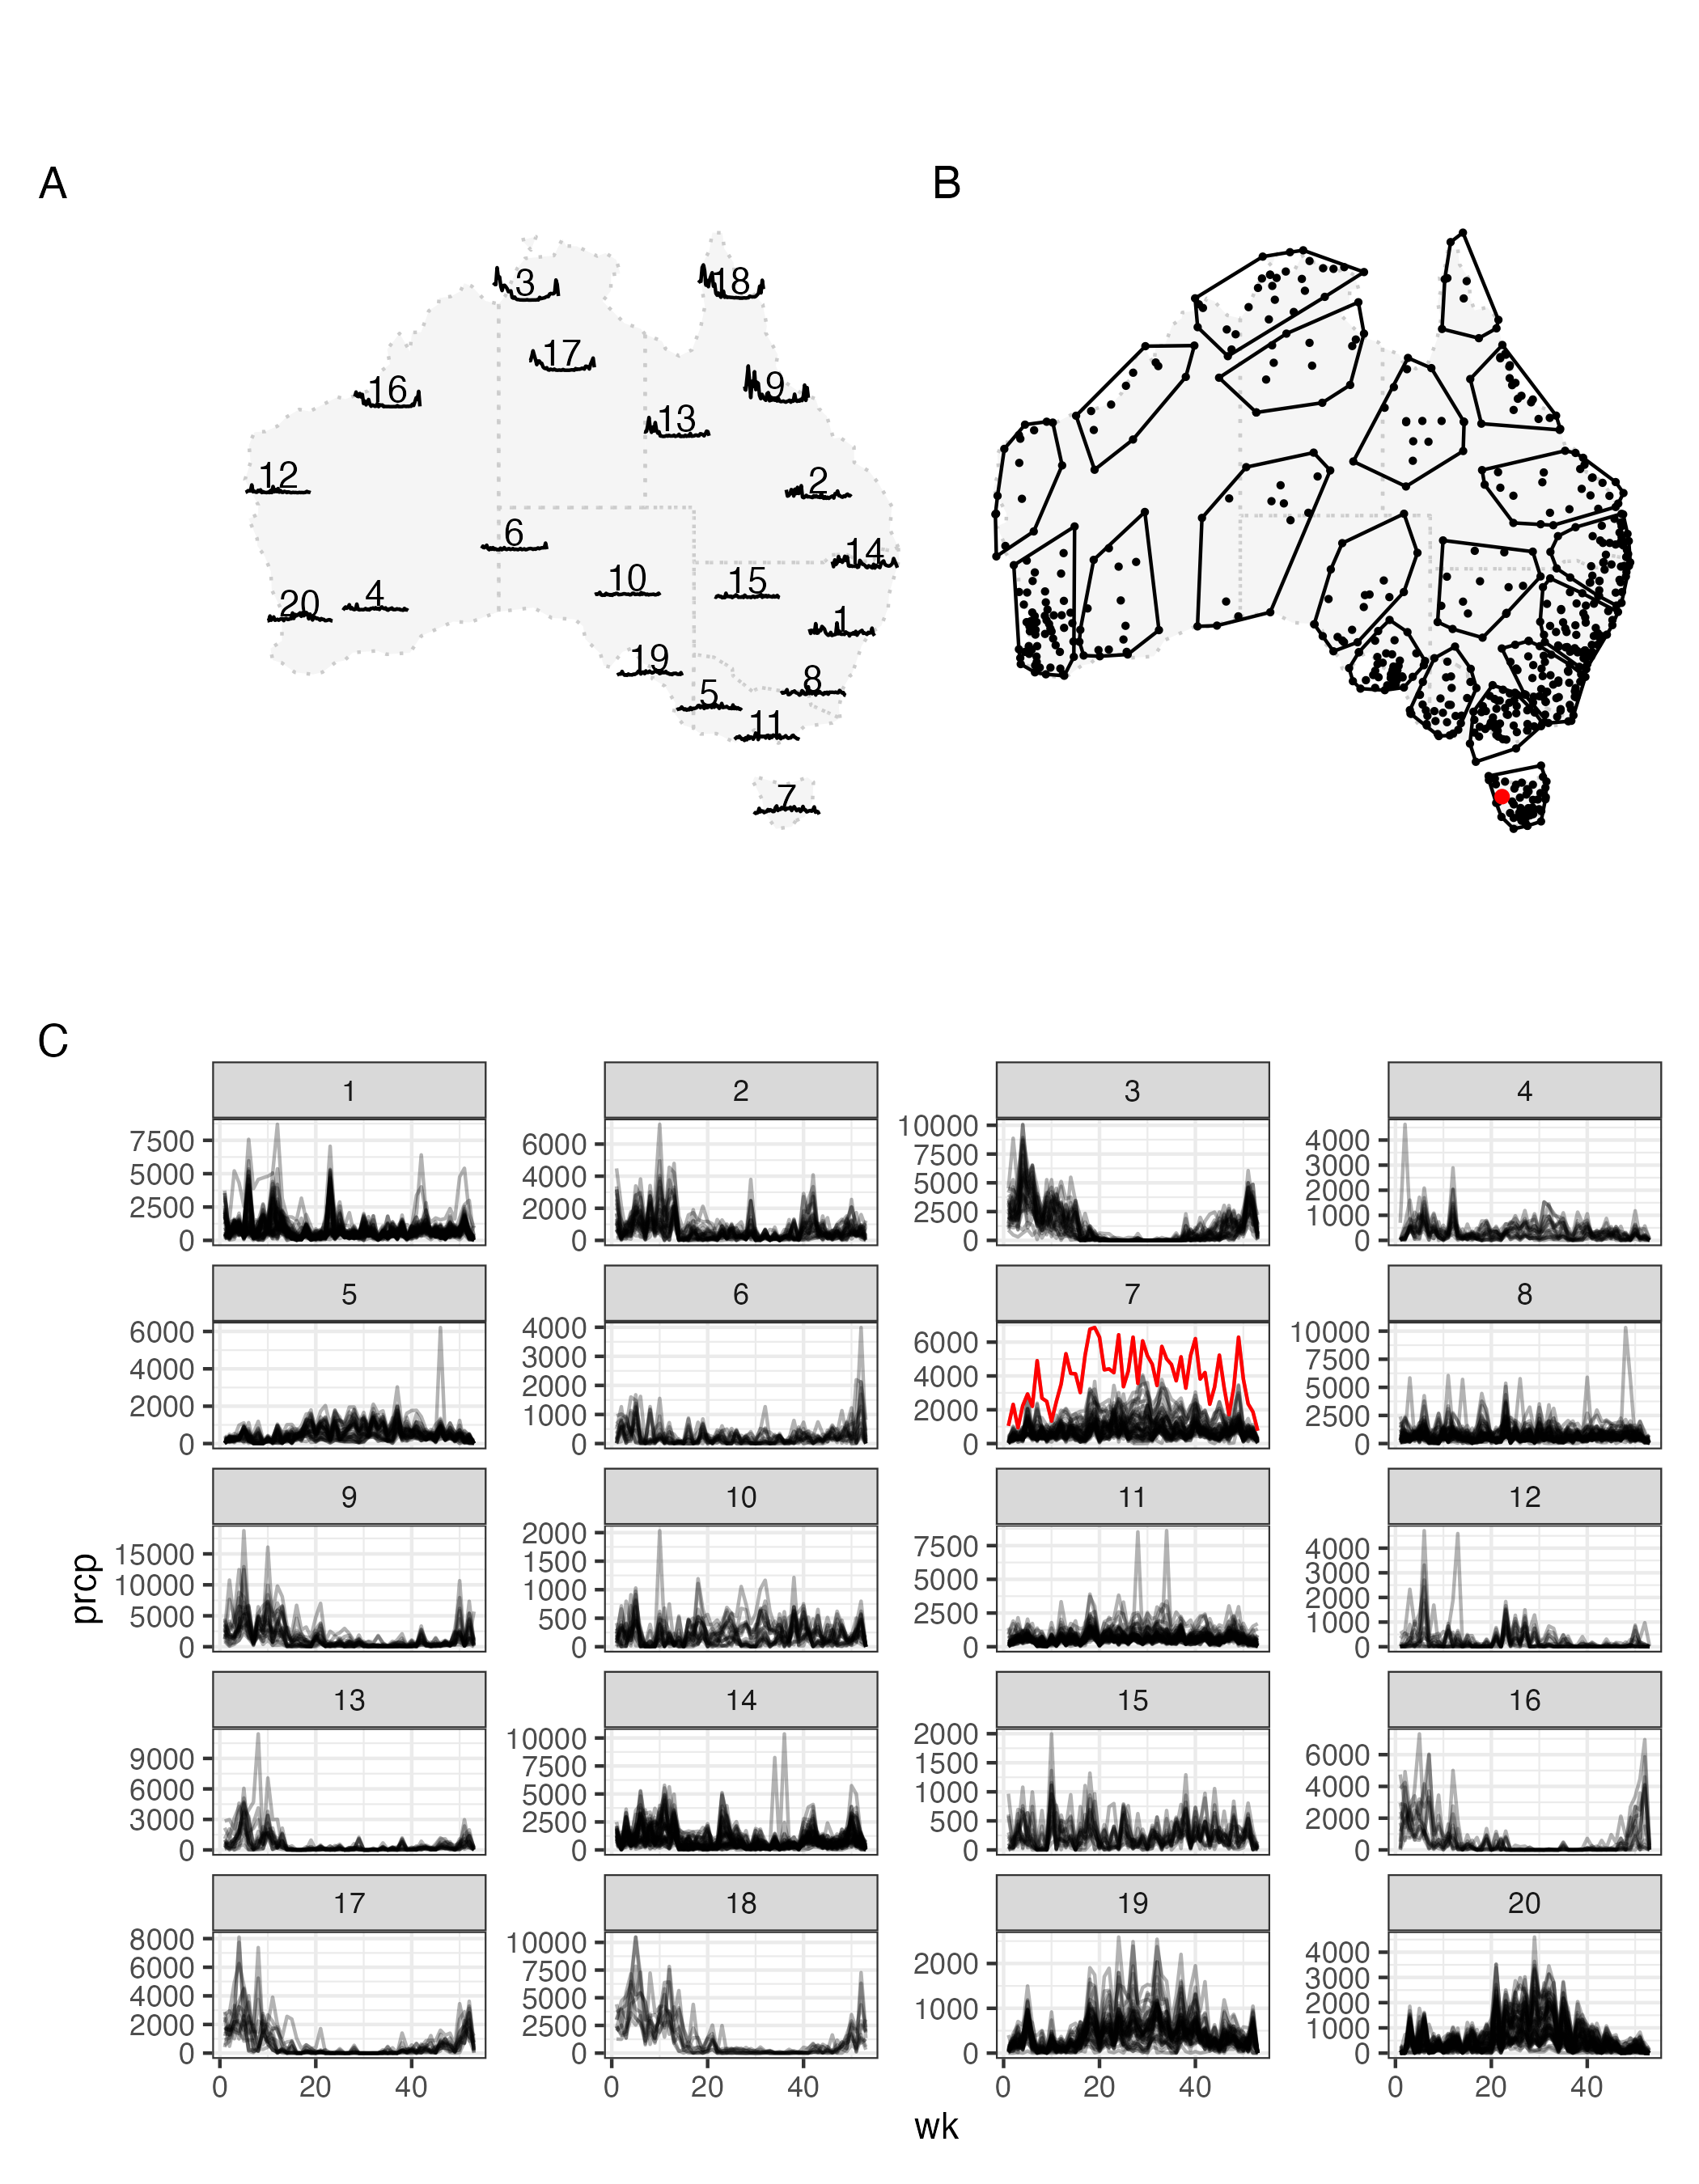
\includegraphics[width=1\linewidth]{/Users/sherryzhang/Documents/research/paper-cubble/figures/basic-agg} \caption{Profile of aggregated precipitation from 639 weather stations in Australia. Subplot A shows the glyph map of the weekly averaged precipitation of each cluster. The group number is printed in the middle of the y minor axis and can be used as a reference line to read the magnitude. Subplot B shows the station membership of each cluster.}\label{fig:basic-agg}
\end{figure}

\hypertarget{river-level-data-in-victoria-water-gauges}{%
\subsection{River level data in Victoria water gauges}\label{river-level-data-in-victoria-water-gauges}}

The Bureau of Meteorology collects \href{http://www.bom.gov.au/metadata/catalogue/19115/ANZCW0503900528?template=full}{water data} from river gauges. The collected variables include: electrical conductivity, turbidity, watercourse discharge, watercourse level, and water temperature. In particular, water level will interact with precipitation from the climate data since rainfall will raise the water level in the river. Figure \ref{fig:matching-map} gives the location of available weather stations and water gauges in Victoria.

\begin{figure}
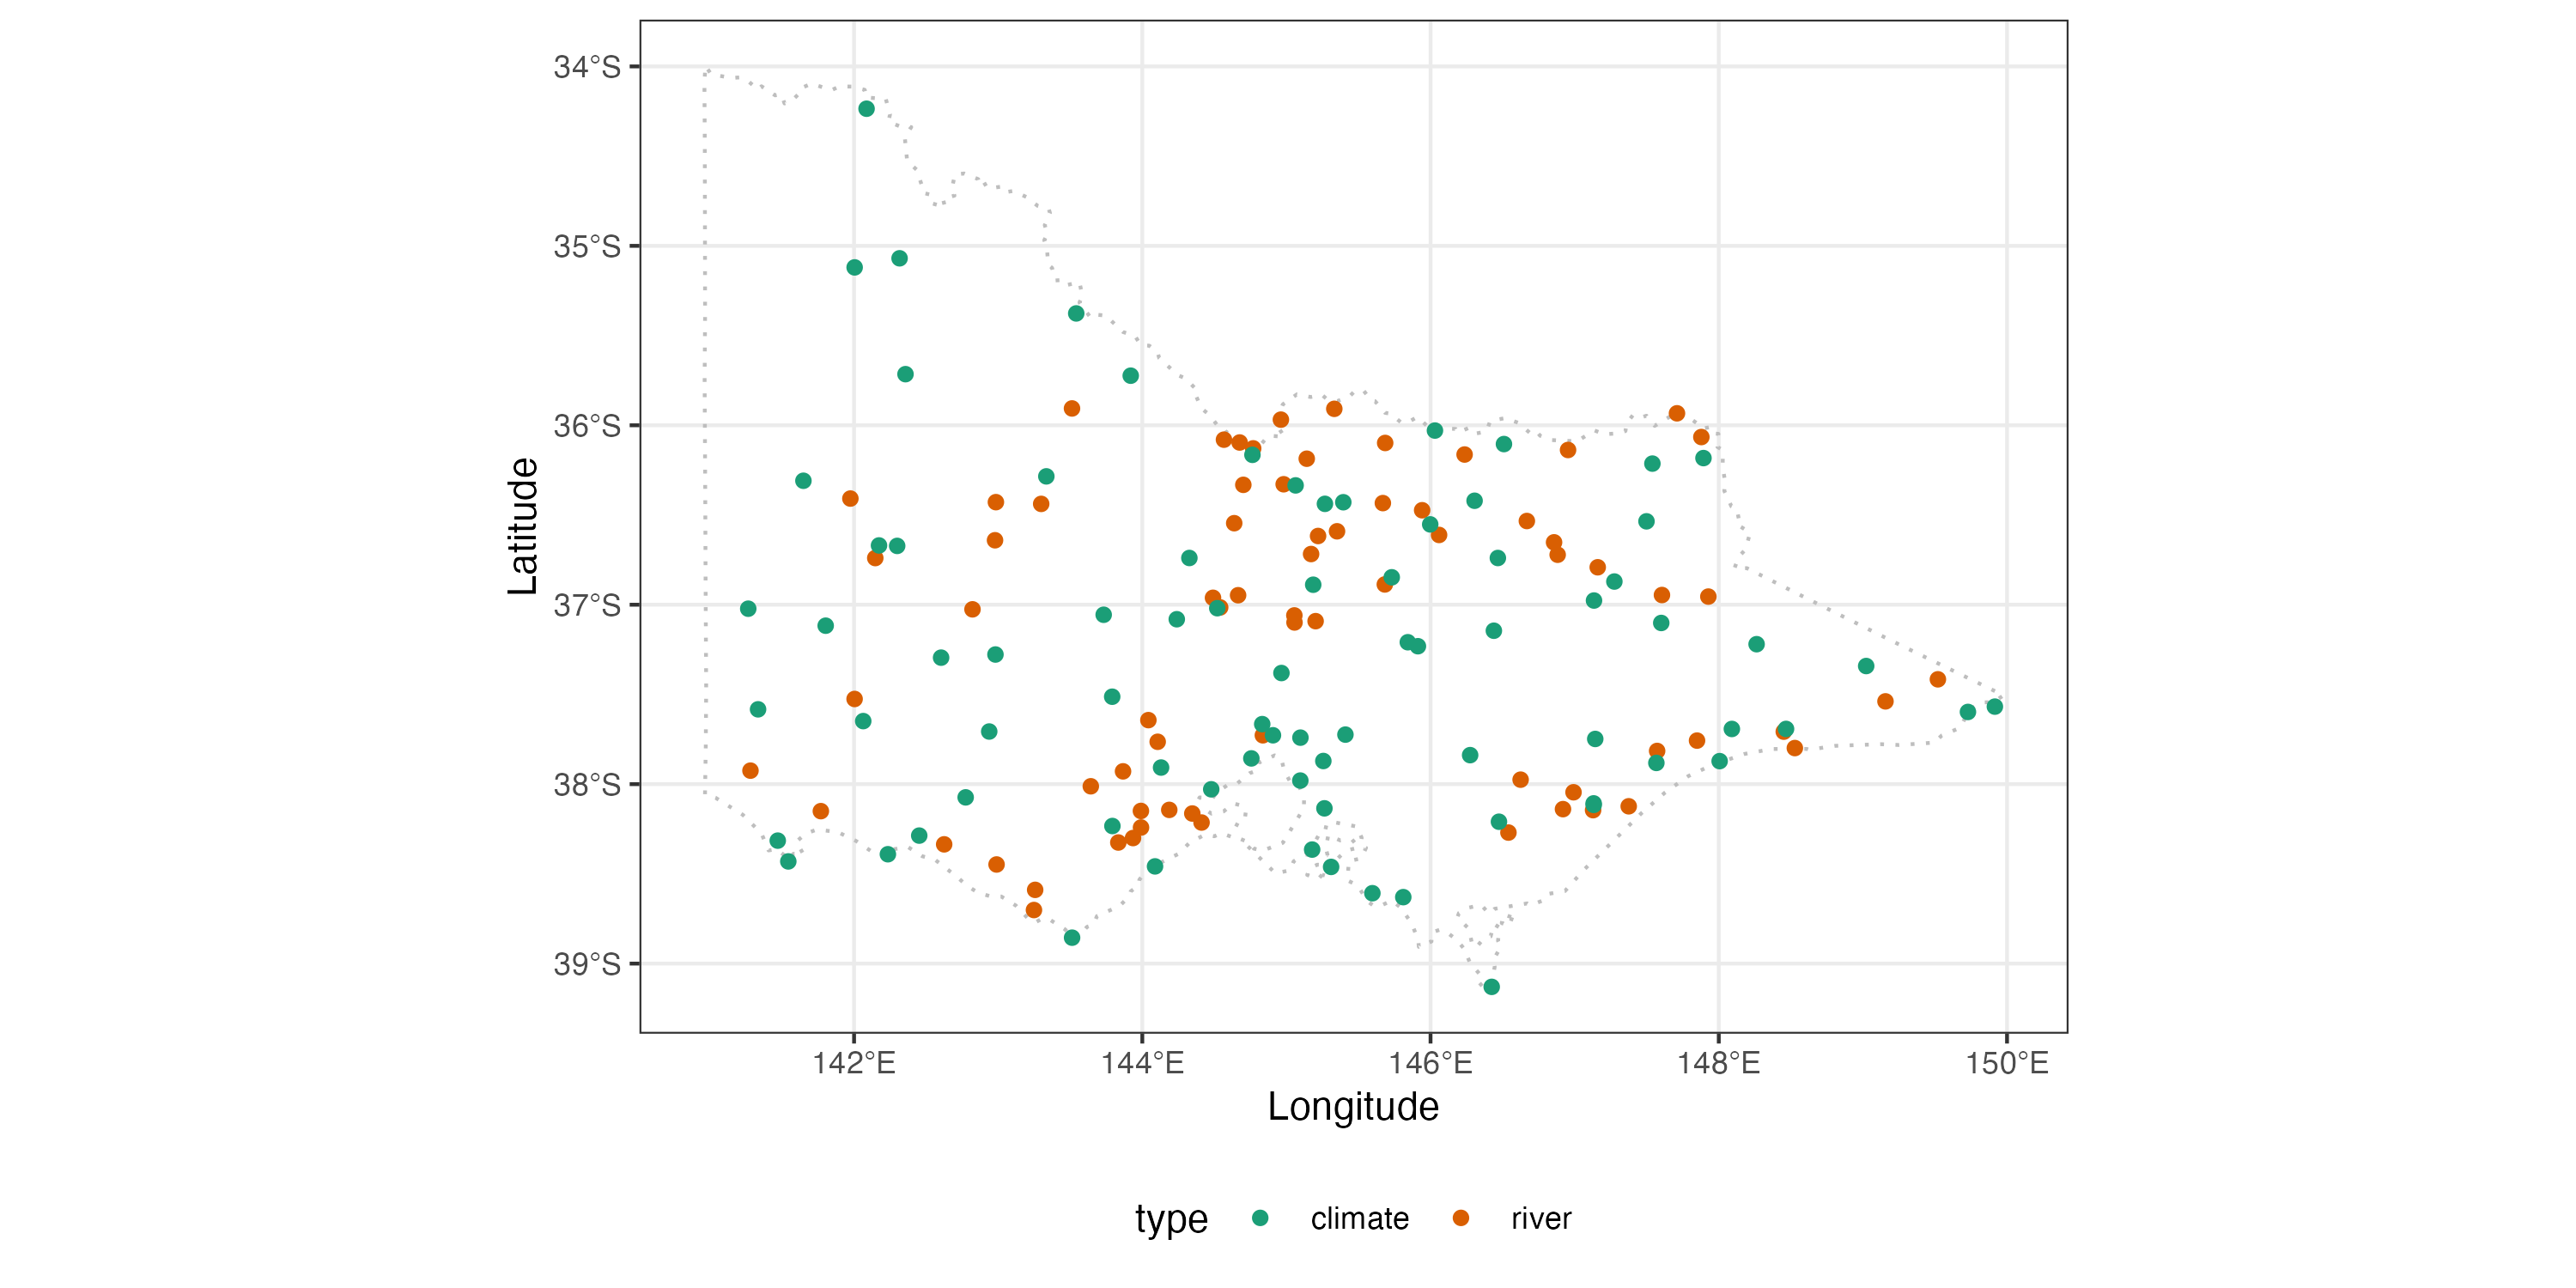
\includegraphics[width=1\linewidth]{/Users/sherryzhang/Documents/research/paper-cubble/figures/matching-map} \caption{Location of weather stations and river gauges in Victoria, Australia.}\label{fig:matching-map}
\end{figure}

From the map, one can see that a few water gauges and weather stations are close to each other and the fluctuation of the water level could be matched up with the precipitation measured by the nearby climate station. As introduced in Section \ref{matching}, \code{match_sites()} can be used to match one source of data with another source in a cubble. Here \code{Water_course_level} in \code{river} will be matched to \code{prcp} in \code{climate} in 2020. The two datasets need to be specified as the first two arguments and the variable to match can be specified in \code{temporal_by} using the \code{by} syntax in \code{join}. \code{temporal_independent} controls the variable used to construct the interval and the goal here is to see if the water level in the river will reflect precipitation. This puts precipitation \code{prcp}, as the independent variable. Given there is one year's worth of data, the number of peaks (\code{temporal_n_highest}) to consider is slightly raised from a default of 20 to 30 and \code{temporal_min_match} is raised accordingly. To return all the pairs of the match, \code{temporal_min_match} can be set to 0.

\begin{Shaded}
\begin{Highlighting}[]
\NormalTok{res }\OtherTok{\textless{}{-}} \FunctionTok{match\_sites}\NormalTok{(}
\NormalTok{  river, climate,}
  \AttributeTok{temporal\_by =} \FunctionTok{c}\NormalTok{(}\StringTok{"Water\_course\_level"} \OtherTok{=} \StringTok{"prcp"}\NormalTok{),}
  \AttributeTok{temporal\_independent =} \StringTok{"prcp"}\NormalTok{,  }
  \AttributeTok{temporal\_n\_highest =} \DecValTok{30}\NormalTok{,}
  \AttributeTok{temporal\_min\_match =} \DecValTok{15}
\NormalTok{)}
\end{Highlighting}
\end{Shaded}

The output from matching is also a cubble, with additional column \code{dist} and \code{group} produced from spatial matching and \code{n_match} from temporal matching.

\begin{verbatim}
## # cubble:   id [8]: nested form
## # bbox:     [144.52, -37.73, 146.06, -36.55]
## # temporal: date [date], matched_var [dbl]
##   id          name                  lat  long type   dist group ts       n_match
##   <chr>       <chr>               <dbl> <dbl> <chr> <dbl> <int> <list>     <int>
## 1 405234      SEVEN CREEKS @ D/S~ -36.9  146. river  6.15     5 <tibble>      21
## 2 404207      HOLLAND CREEK @ KE~ -36.6  146. river  8.54    10 <tibble>      21
## 3 ASN00082042 strathbogie         -36.8  146. clim~  6.15     5 <tibble>      21
## 4 ASN00082170 benalla airport     -36.6  146. clim~  8.54    10 <tibble>      21
## 5 230200      MARIBYRNONG RIVER ~ -37.7  145. river  6.17     6 <tibble>      19
## 6 ASN00086038 essendon airport    -37.7  145. clim~  6.17     6 <tibble>      19
## 7 406213      CAMPASPE RIVER @ R~ -37.0  145. river  1.84     1 <tibble>      18
## 8 ASN00088051 redesdale           -37.0  145. clim~  1.84     1 <tibble>      18
\end{verbatim}

Figure \ref{fig:matching} plots the matched pairs on the map. There are four pairs of matches, all located in the middle of Victoria and the expected concurrent increase in precipitation and water level can be observed.

\begin{figure}
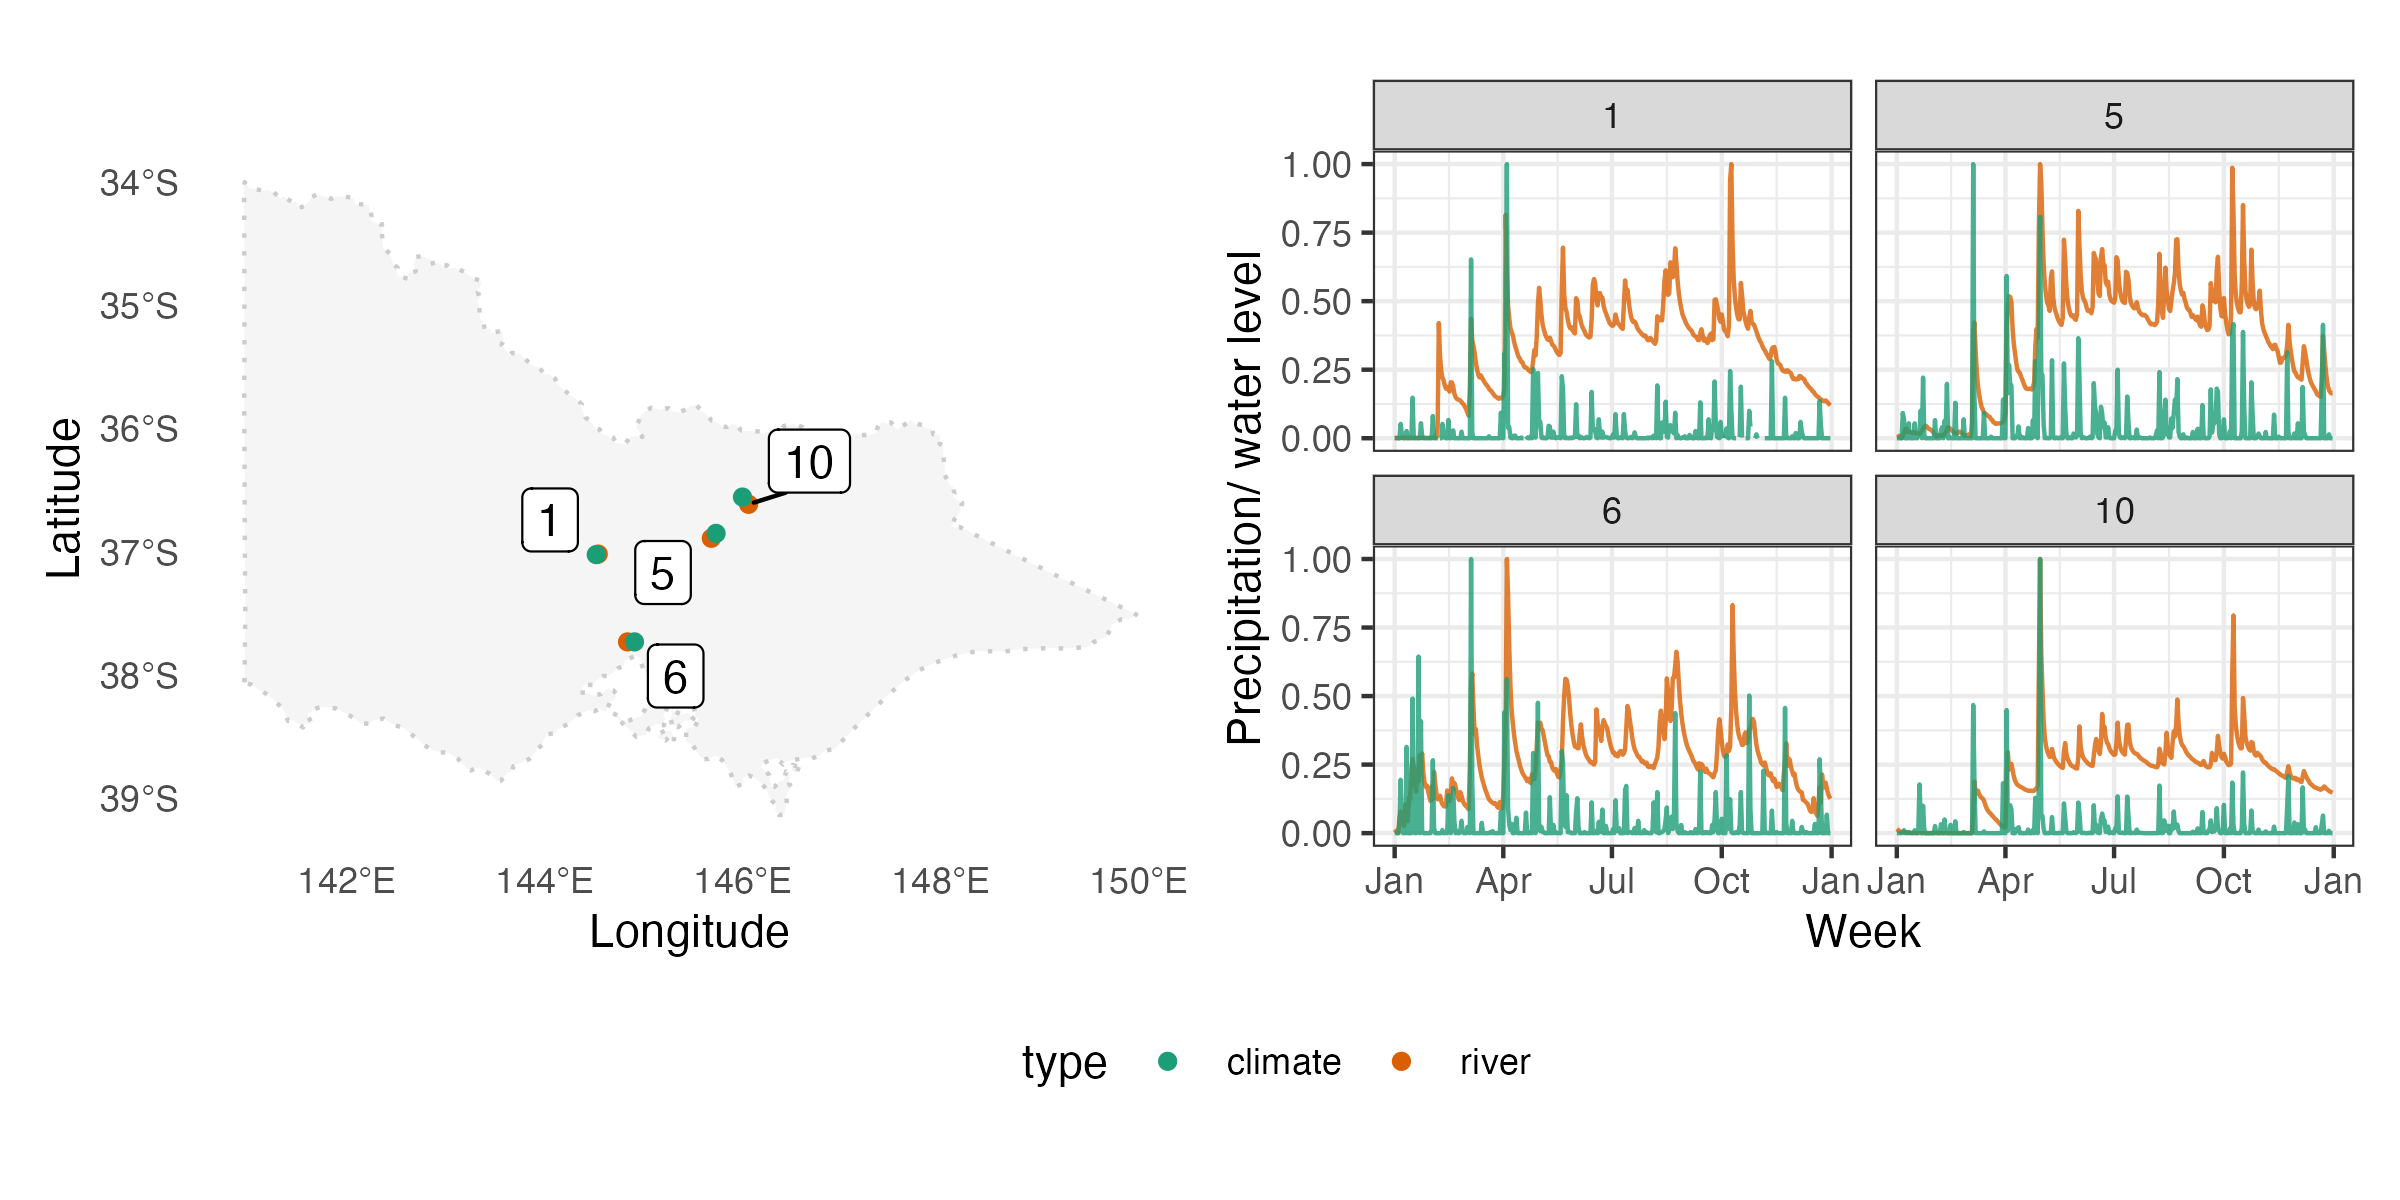
\includegraphics[width=1\linewidth]{/Users/sherryzhang/Documents/research/paper-cubble/figures/matching} \caption{Matched weather stations and river gauges on the map (A) and across time (B). Precipitation and water level have been standardised between 0 and 1 to be displayed on the same scale. The water level reflects the increase in precipitation.}\label{fig:matching}
\end{figure}

\hypertarget{era5-climate-reanalysis-data}{%
\subsection{ERA5: climate reanalysis data}\label{era5-climate-reanalysis-data}}

The ERA5 dataset (\protect\hyperlink{ref-hersbach2020era5}{Hersbach et al. 2020}) is the latest reanalysis of global atmosphere, land surface, and ocean waves from 1950 onwards and is available in the NetCDF format from the European Centre for Medium-Range Weather Forecasts (ECMWF). The data can be directly downloaded from \href{https://cds.climate.copernicus.eu/cdsapp\#!/dataset/reanalysis-era5-pressure-levels?tab=overview}{Copernicus Climate Data Store (CDS)} website or programmatically via the R package \pkg{ecmwfr} (\protect\hyperlink{ref-ecwmfr}{Hufkens, Stauffer, and Campitelli 2019}). The \code{era5-pressure} data contains the \emph{specific humidity} and \emph{geopotential} variables on the 10 hPa pressure level on four dates: 2002-09-22, 2002-09-26, 2002-09-30, and 2002-10-04. Once downloaded, the data can be read into a cubble as:

\begin{Shaded}
\begin{Highlighting}[]
\NormalTok{raw }\OtherTok{\textless{}{-}}\NormalTok{ ncdf4}\SpecialCharTok{::}\FunctionTok{nc\_open}\NormalTok{(here}\SpecialCharTok{::}\FunctionTok{here}\NormalTok{(}\StringTok{"data/era5{-}pressure.nc"}\NormalTok{))}
\NormalTok{dt }\OtherTok{\textless{}{-}} \FunctionTok{as\_cubble}\NormalTok{(raw, }\AttributeTok{vars =} \FunctionTok{c}\NormalTok{(}\StringTok{"q"}\NormalTok{, }\StringTok{"z"}\NormalTok{))}
\end{Highlighting}
\end{Shaded}

Figure \ref{fig:netcdf} reproduces the ERA5 data row of Figure 19 in Hersbach et al. (\protect\hyperlink{ref-hersbach2020era5}{2020}). It shows the southern polar vortex splits into two on 2002-09-26 and further splits into four on 2002-10-04 in the stratosphere. Readers interested in the analysis of this figure can refer to Hersbach et al. (\protect\hyperlink{ref-hersbach2020era5}{2020}), Simmons et al. (\protect\hyperlink{ref-simmons2020global}{2020}), and Simmons et al. (\protect\hyperlink{ref-simmons2005ecmwf}{2005}) for more details.

\begin{figure}
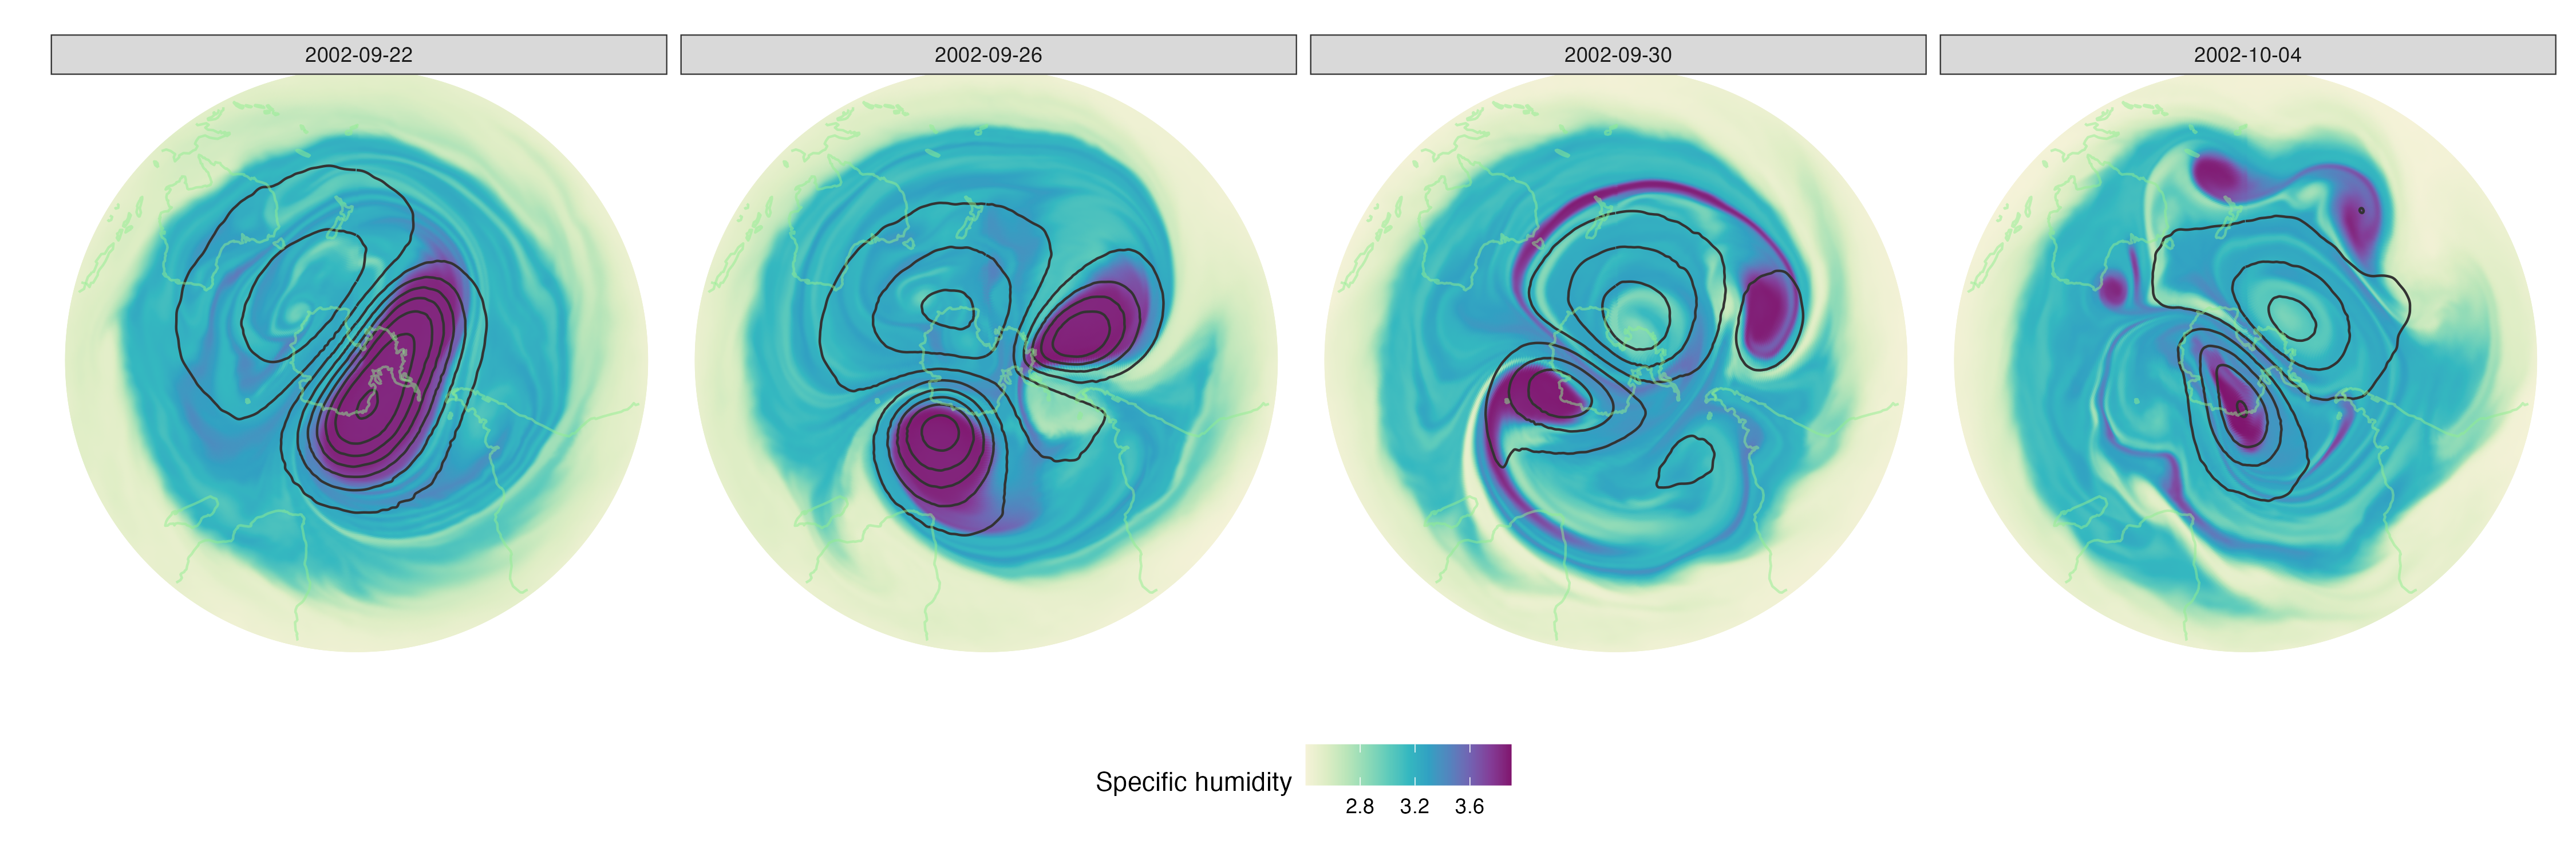
\includegraphics[width=1\linewidth]{/Users/sherryzhang/Documents/research/paper-cubble/figures/netcdf} \caption{A reproduction of the second row (ERA5 data) of Figure 19 in Hersbach et al (2020).}\label{fig:netcdf}
\end{figure}

\hypertarget{interactive-graphic}{%
\subsection{Interactive graphic}\label{interactive-graphic}}

With spatio-temporal data, users may wish to make plots to learn the spatial distribution of a variable or to find patterns, such as trend or seasonality, in the time series. Combining these two types of plots with interactivity lets users link between points on the map and the corresponding time series to explore the spatial and temporal dimensions of the data simultaneously. Below is an example that describes the process of building an interactive graphic with \pkg{cubble} and \pkg{crosstalk}. The example explores the variation of monthly temperature range with \code{weatherdata::climate_full} data.

The temperature range is calculated as the difference between \code{tmax} and \code{tmin} and its monthly average over 2016-2020 is taken before calculating the variance. A \code{SharedData} object is constructed for each form of the cubble and the same \code{group} argument ensures the cross-linking of the two forms via the common \code{id} column. The spatial map and time series plot are then made with each \code{SharedData} object separately. In this example, stations on the Australia map, made from the nested form, are coloured by the calculated variance. A ribbon band is constructed using the long form cubble to show each station's maximum and minimum temperature across month. With a different dataset, users can calculate other per station measure in the nested form or make other time-wise summary of the data in the long form to customise the spatial or temporal view. The cross-linking between the two plots is always safeguarded by the shared \code{id} column embedded in the cubble structure. Below is the pseudo-code that outlines the process to construct an interactive graphic described above:

\begin{Shaded}
\begin{Highlighting}[]
\CommentTok{\# data pre{-}processing}
\NormalTok{clean }\OtherTok{\textless{}{-}}\NormalTok{ weatherdata}\SpecialCharTok{::}\NormalTok{climate\_full }\SpecialCharTok{|\textgreater{}}\NormalTok{ ...}

\CommentTok{\# created SharedData instance for crosstalk}
\NormalTok{nested }\OtherTok{\textless{}{-}}\NormalTok{ clean }\SpecialCharTok{|\textgreater{}}\NormalTok{ SharedData}\SpecialCharTok{$}\FunctionTok{new}\NormalTok{(}\SpecialCharTok{\textasciitilde{}}\NormalTok{id, }\AttributeTok{group =} \StringTok{"cubble"}\NormalTok{)}
\NormalTok{long }\OtherTok{\textless{}{-}} \FunctionTok{face\_temporal}\NormalTok{(clean) }\SpecialCharTok{|\textgreater{}}\NormalTok{ SharedData}\SpecialCharTok{$}\FunctionTok{new}\NormalTok{(}\SpecialCharTok{\textasciitilde{}}\NormalTok{id, }\AttributeTok{group =} \StringTok{"cubble"}\NormalTok{)}

\CommentTok{\# create the spatial and temporal view each with a ShareData instance}
\NormalTok{p1 }\OtherTok{\textless{}{-}}\NormalTok{ nested }\SpecialCharTok{|\textgreater{}}\NormalTok{ ...}
\NormalTok{p2 }\OtherTok{\textless{}{-}}\NormalTok{ long }\SpecialCharTok{|\textgreater{}}\NormalTok{ ...}

\CommentTok{\# Combine p1 and p2}
\NormalTok{crosstalk}\SpecialCharTok{::}\FunctionTok{bscols}\NormalTok{(plotly}\SpecialCharTok{::}\FunctionTok{ggplotly}\NormalTok{(p1), plotly}\SpecialCharTok{::}\FunctionTok{ggplotly}\NormalTok{(p2), ...)}
\end{Highlighting}
\end{Shaded}

In Figure \ref{fig:interactive-linking}, the first row shows the initial view of the interactive graphic. Most regions in Australia have low variance of temperature range, while the north-west coastline, bottom of South Australia, and Victoria stand out with larger monthly changes. In the second row, Mount Elizabeth is selected on the map given its high variance colour on the initial map and this links to the ribbon on the right. The third row selects the lowest temperature in August and this corresponds to Thredbo AWS on the Victoria and New South Wales border. Another station in the Tasmania island is selected on the map to cross compare with Thredbo AWS.

\begin{figure}
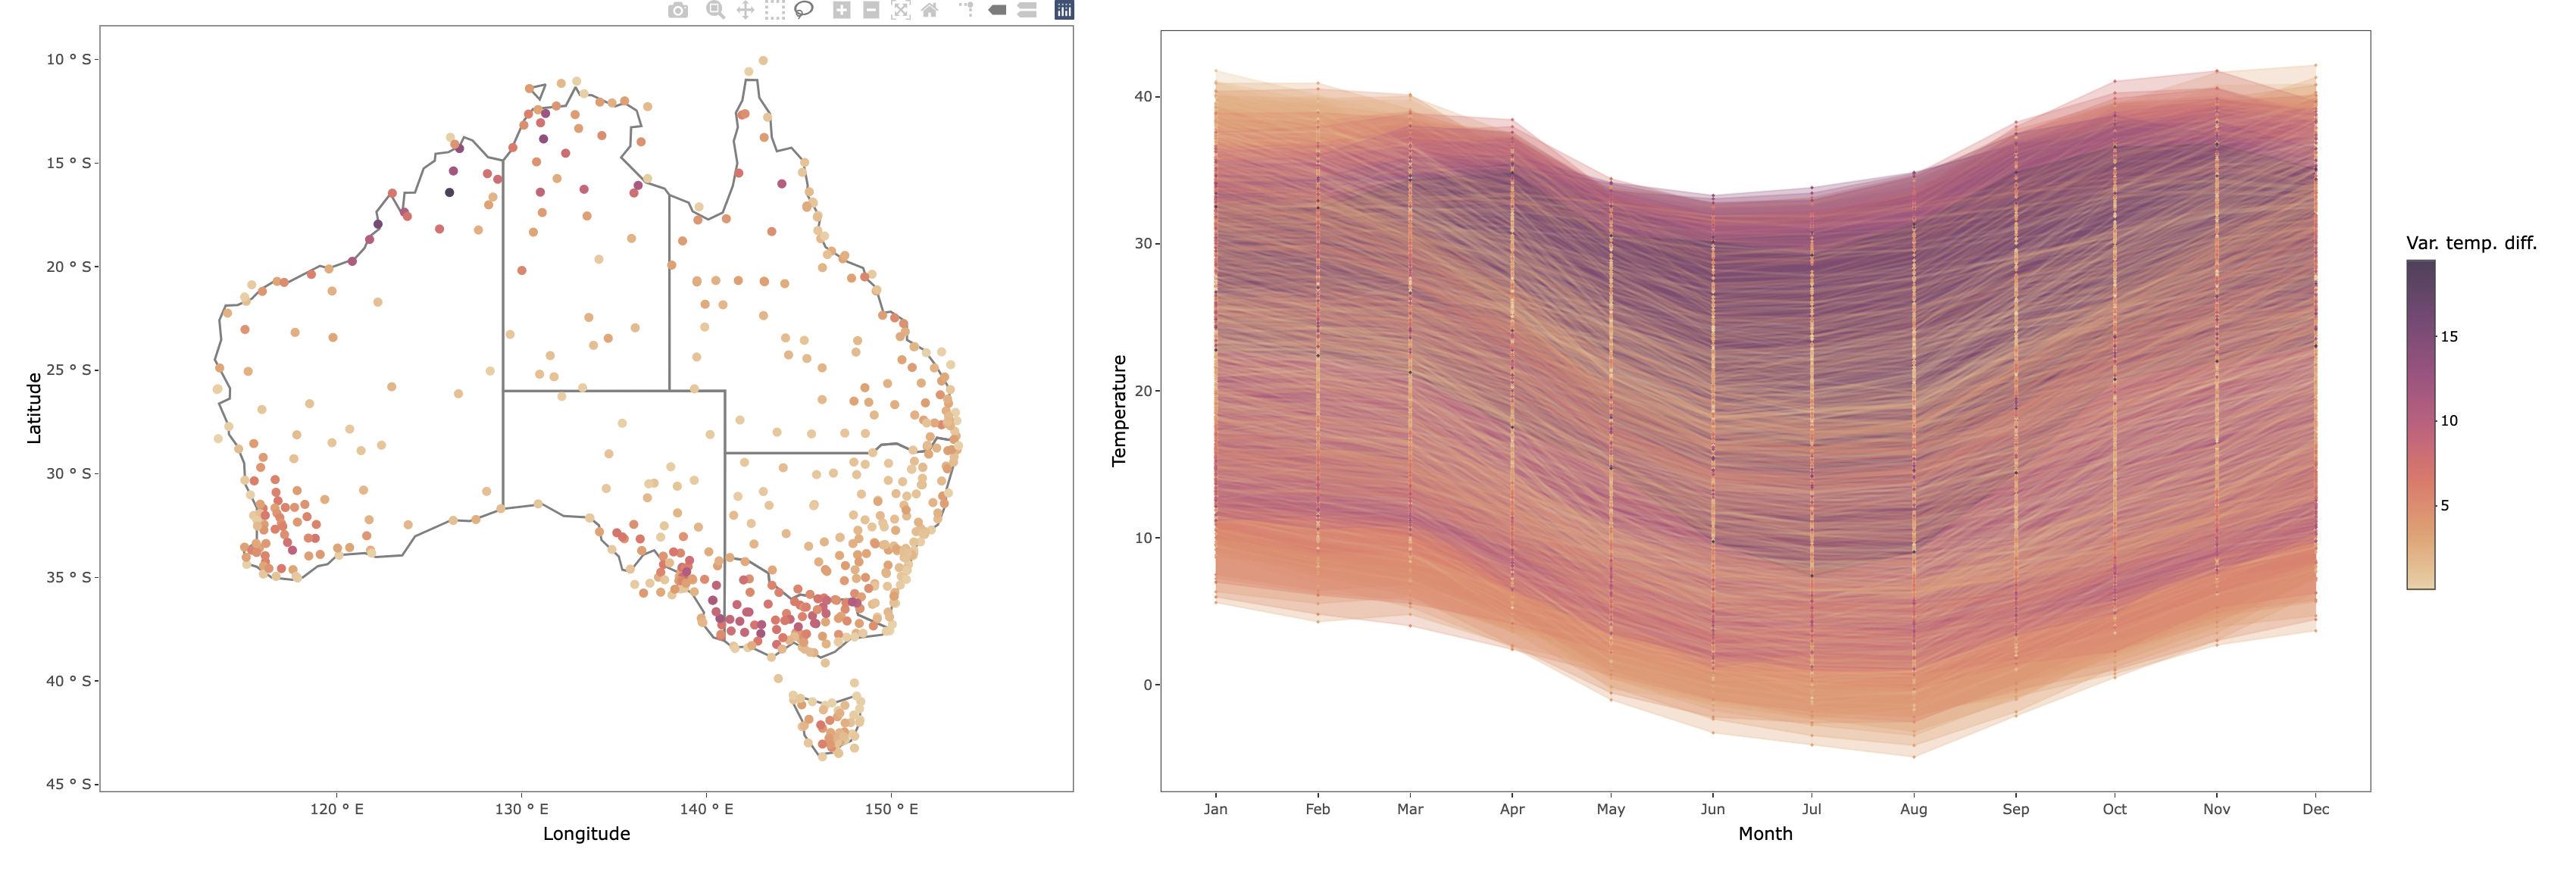
\includegraphics[width=1\linewidth,height=0.23\textheight]{/Users/sherryzhang/Documents/research/paper-cubble/figures/linking} 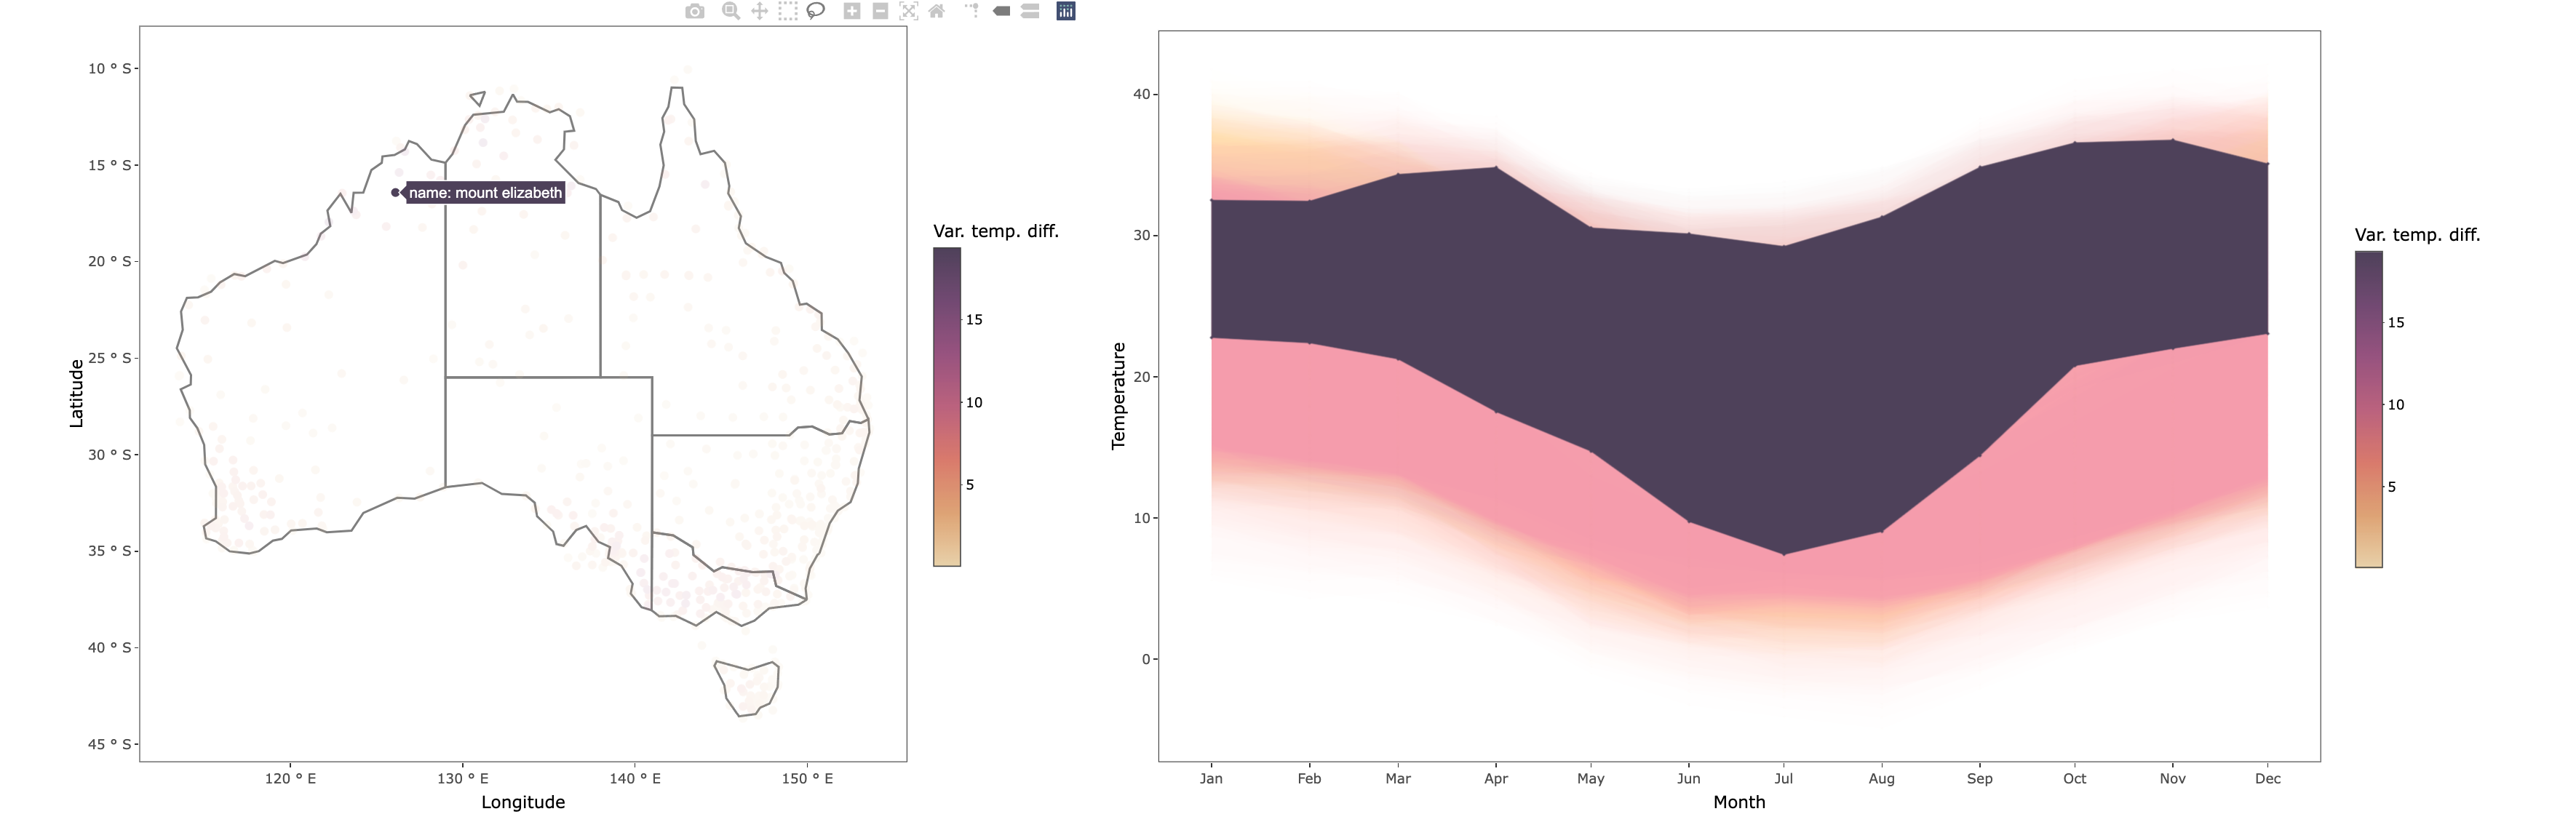
\includegraphics[width=1\linewidth,height=0.23\textheight]{/Users/sherryzhang/Documents/research/paper-cubble/figures/linking-north} 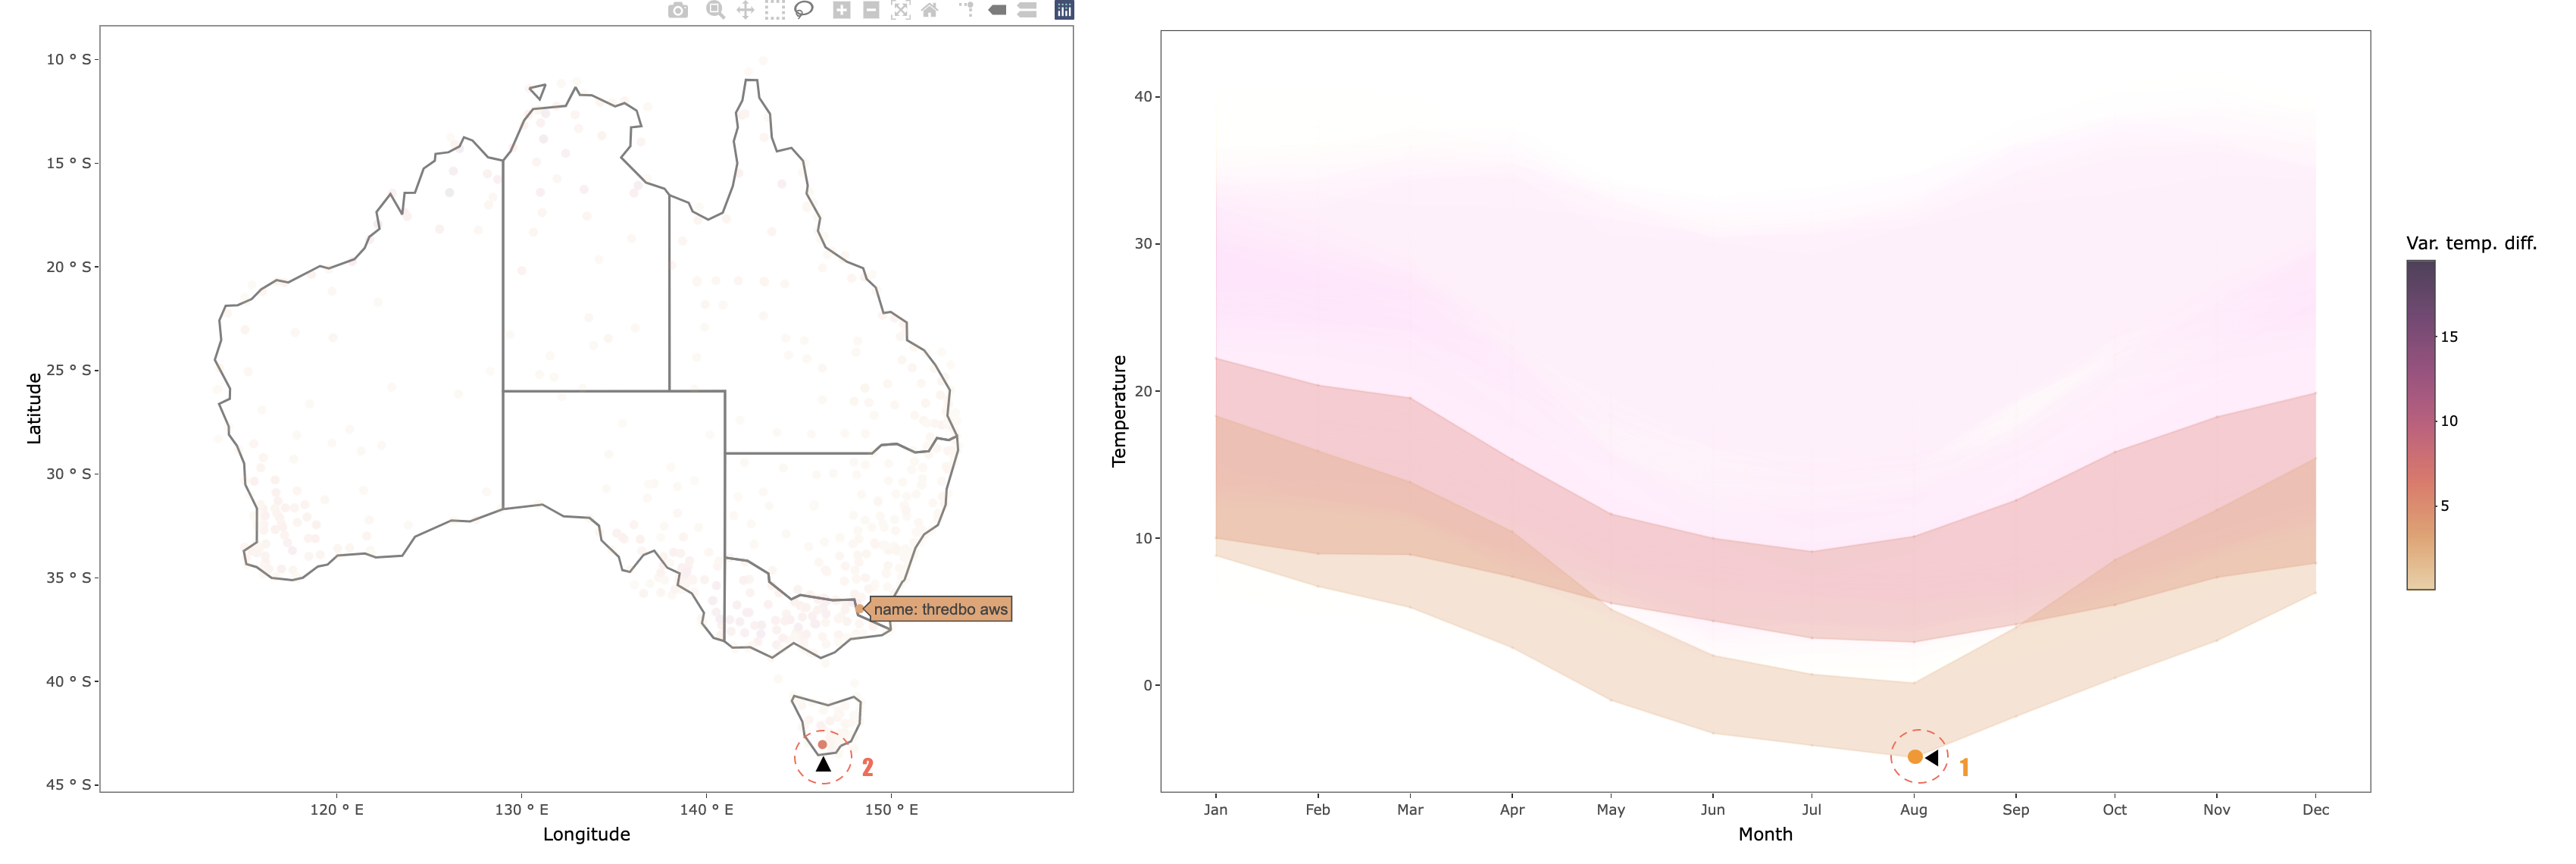
\includegraphics[width=1\linewidth,height=0.23\textheight]{/Users/sherryzhang/Documents/research/paper-cubble/figures/linking-lower} \caption{Exploring temperature variation using linking of a map and seasonal display. Each row is a screen dump of the process. The top row shows all locations and all temperature profiles. Selecting a location with high variance on the map produces the plot in the second row. The maximum and minimum temperature is shown using a ribbon. The bottom row first selects the lowest temperature in August in the seasonal display. A location in the Tasmania Island is then selected to compare the temperature variation with Thredbo AWS.}\label{fig:interactive-linking}
\end{figure}

This plot can also be made using \pkg{cubble} and \pkg{leaflet} where the temperature range is displayed as a small subplot upon clicking on the map. The procedure involves first creating the popup plots from the long form cubble as a vector and then adding these plots to a leaflet map created from the nested cubble, with \code{leafpop::addPopupGraphs()}:

\begin{Shaded}
\begin{Highlighting}[]
\CommentTok{\# data pre{-}processing}
\NormalTok{clean }\OtherTok{\textless{}{-}}\NormalTok{ weatherdata}\SpecialCharTok{::}\NormalTok{climate\_full }\SpecialCharTok{|\textgreater{}}\NormalTok{ ...}

\CommentTok{\# use the long form to create subplots for each station}
\NormalTok{df\_id }\OtherTok{\textless{}{-}} \FunctionTok{unique}\NormalTok{(clean}\SpecialCharTok{$}\NormalTok{id)}
\NormalTok{p }\OtherTok{\textless{}{-}} \FunctionTok{map}\NormalTok{(}\DecValTok{1}\SpecialCharTok{:}\FunctionTok{length}\NormalTok{(df\_id), }\ControlFlowTok{function}\NormalTok{(i)\{}
\NormalTok{  dt }\OtherTok{\textless{}{-}}\NormalTok{ clean }\SpecialCharTok{|\textgreater{}} \FunctionTok{filter}\NormalTok{(id }\SpecialCharTok{==}\NormalTok{ df\_id[i])}
  \FunctionTok{ggplot}\NormalTok{(dt) }\SpecialCharTok{|\textgreater{}}\NormalTok{ ...}
\NormalTok{\})}

\CommentTok{\# create nested form leaflet map with temperature band as subplots}
\NormalTok{nested }\OtherTok{\textless{}{-}} \FunctionTok{face\_spatial}\NormalTok{(clean)}
\FunctionTok{leaflet}\NormalTok{(nested) }\SpecialCharTok{|\textgreater{}}
  \FunctionTok{addTiles}\NormalTok{() }\SpecialCharTok{|\textgreater{}}
  \FunctionTok{addCircleMarkers}\NormalTok{(}\AttributeTok{group =} \StringTok{"a"}\NormalTok{, ...) }\SpecialCharTok{|\textgreater{}}
\NormalTok{  leafpop}\SpecialCharTok{::}\FunctionTok{addPopupGraphs}\NormalTok{(}\AttributeTok{graph =}\NormalTok{ p, ...)}
\end{Highlighting}
\end{Shaded}

Figure \ref{fig:interactive-popup} shows Figure \ref{fig:interactive-linking} made with leaflet and popups (\protect\hyperlink{ref-leafpop}{Appelhans and Detsch 2021}).

\begin{figure}

{\centering 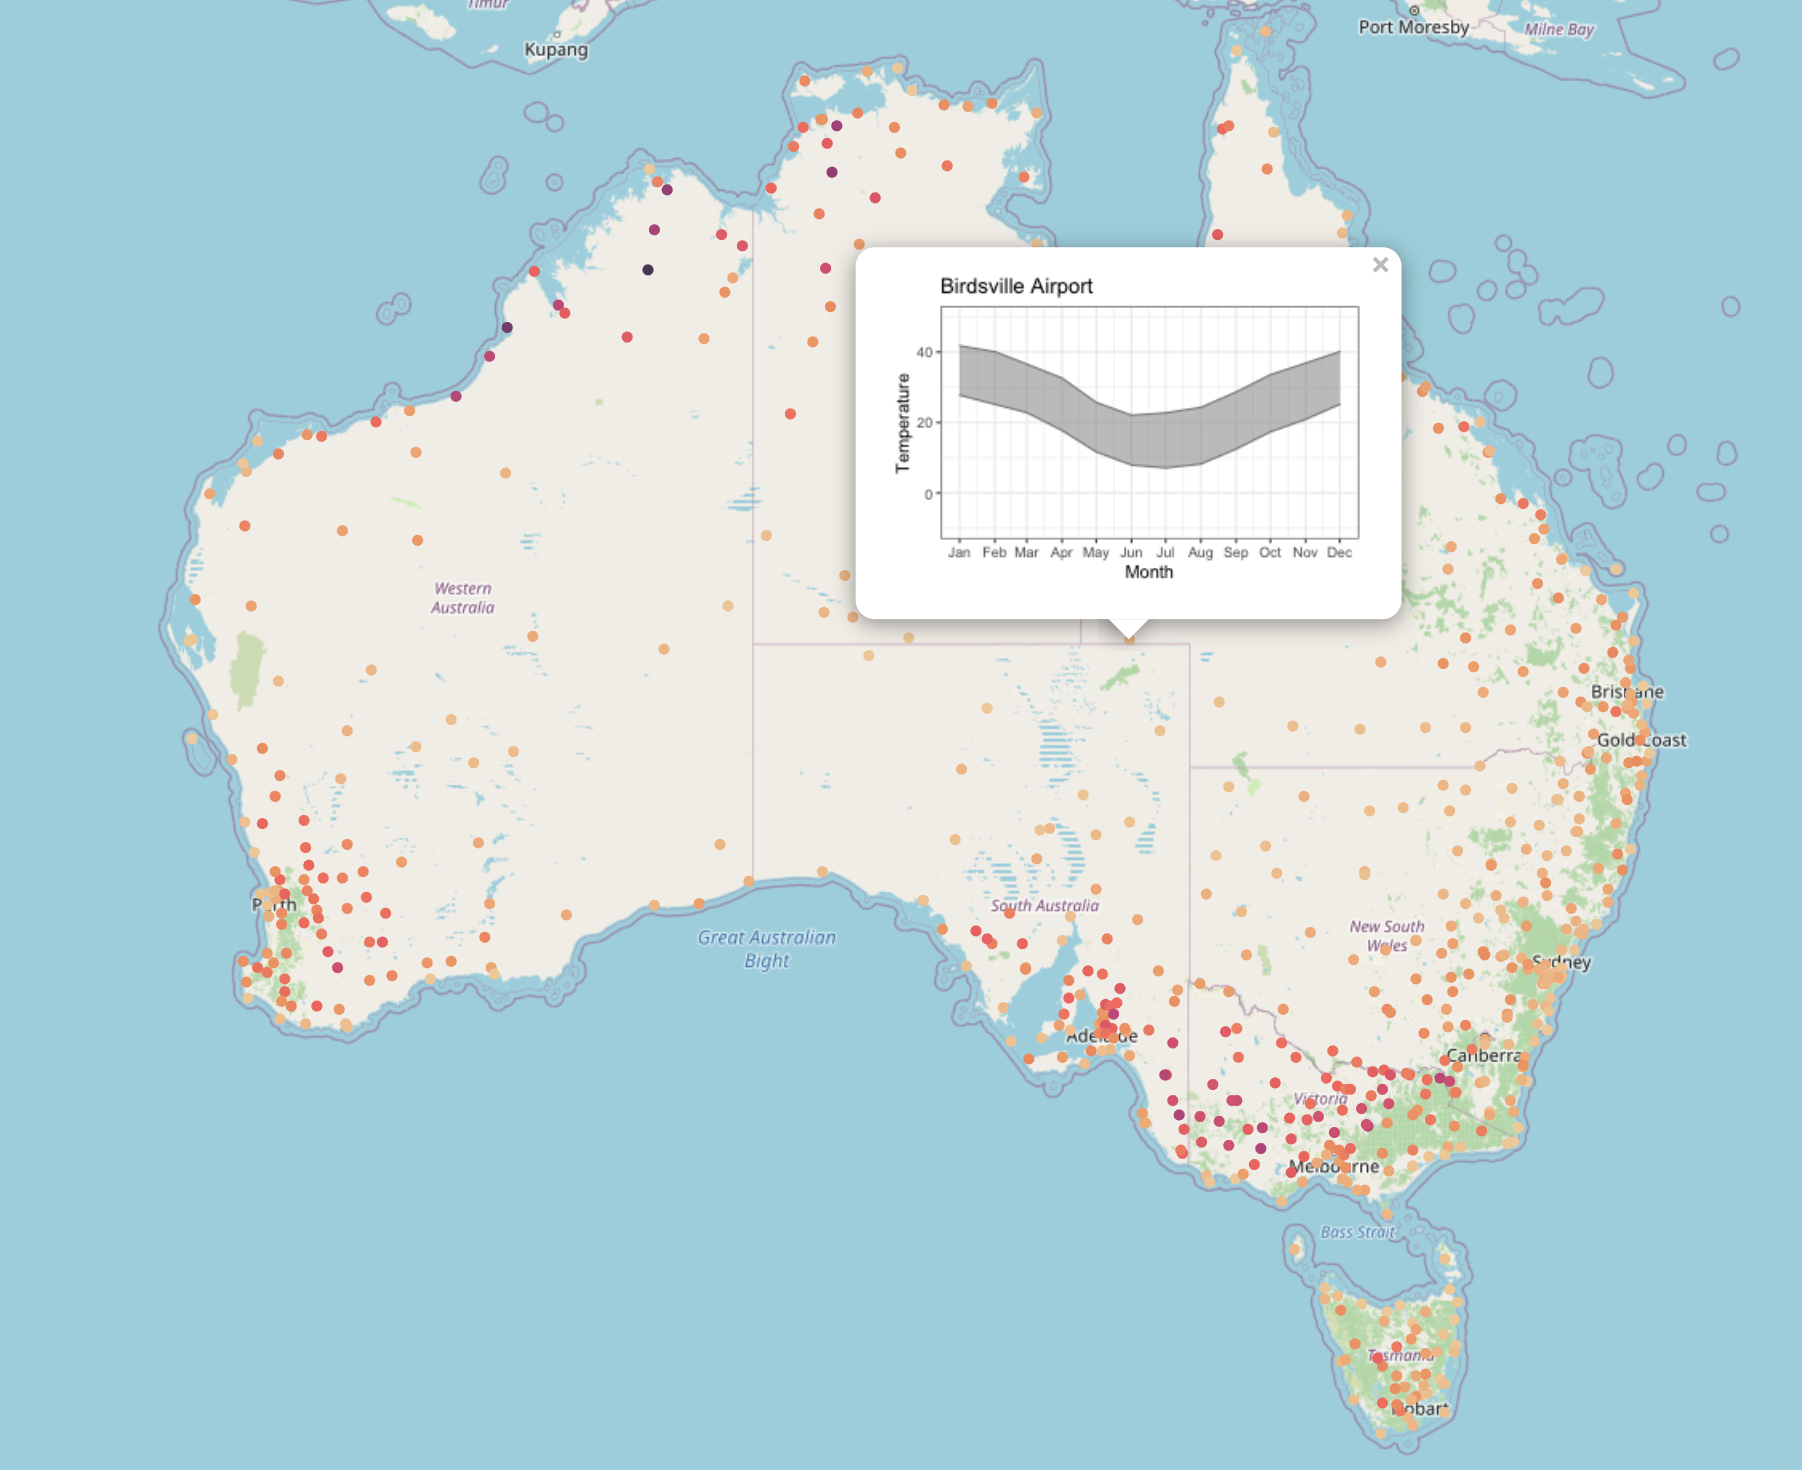
\includegraphics[width=0.45\linewidth,height=0.25\textheight]{/Users/sherryzhang/Documents/research/paper-cubble/figures/popup-mid} 

}

\caption{Same as Figure 11 with the temperature variation shown as a popup in the leaflet map.}\label{fig:interactive-popup}
\end{figure}

\hypertarget{conclude}{%
\section{Conclusion}\label{conclude}}

This paper presents an \proglang{R} package \pkg{cubble} for organising, manipulating and visualising spatio-temporal data. The package introduces a new data structure for spatio-temporal data, \code{cubble}, that connects the time invariant and varying variables and that allows the user to work with a nested and long form of the data. TThe goal of this work is to add capabilities into the spatio-temporal practitioners toolbox that facilitates their work within the tidy data framework. The data structure and the capabilities introduced in this package can be used and combined with existing spatio-temporal R packages such as \pkg{sf}, data wrangling packages such as \pkg{dplyr}, and visualization packages such as \pkg{ggplot2}, \pkg{plotly} and \pkg{leaflet}.

The data structure and functions are demonstrated with extensive examples. These include creating and coercing wild-caught data with potential mismatch on sites, handling hierarchical data, matching time series spatially and temporally, as well as reproducing ERA5 results from NetCDF data. Visualization of the \code{cubble} objects and derivatives is presented via interactive graphic pipelines using \pkg{plotly} and \pkg{leaflet}.

Future directions of the package involves handling sites with moving coordinates. This would involve constructing a list-column for location coordinates and a form these locations can be pivoted into, like the long form for temporal variables. In the multivariate aspect, \pkg{cubble} can also be extended with interface to more high dimensional visualisation methods, i.e., the tour method, to understand variable importance or comparing location similarities.

\newpage

\hypertarget{acknowledgement}{%
\section{Acknowledgement}\label{acknowledgement}}

This work is funded by a Commonwealth Scientific and Industrial Research Organisation (CSIRO) Data61 Scholarship and started while Nicolas Langrené was affiliated with CSIRO's Data61. The article is created using \pkg{knitr} (\protect\hyperlink{ref-knitr}{Xie 2015}) and \pkg{rmarkdown} (\protect\hyperlink{ref-rmarkdown}{Xie, Allaire, and Grolemund 2018}) in R. The source code for reproducing this paper can be found at: \url{https://github.com/huizezhang-sherry/paper-cubble}.

\hypertarget{appendix}{%
\section{Appendix}\label{appendix}}

\begin{figure}

{\centering 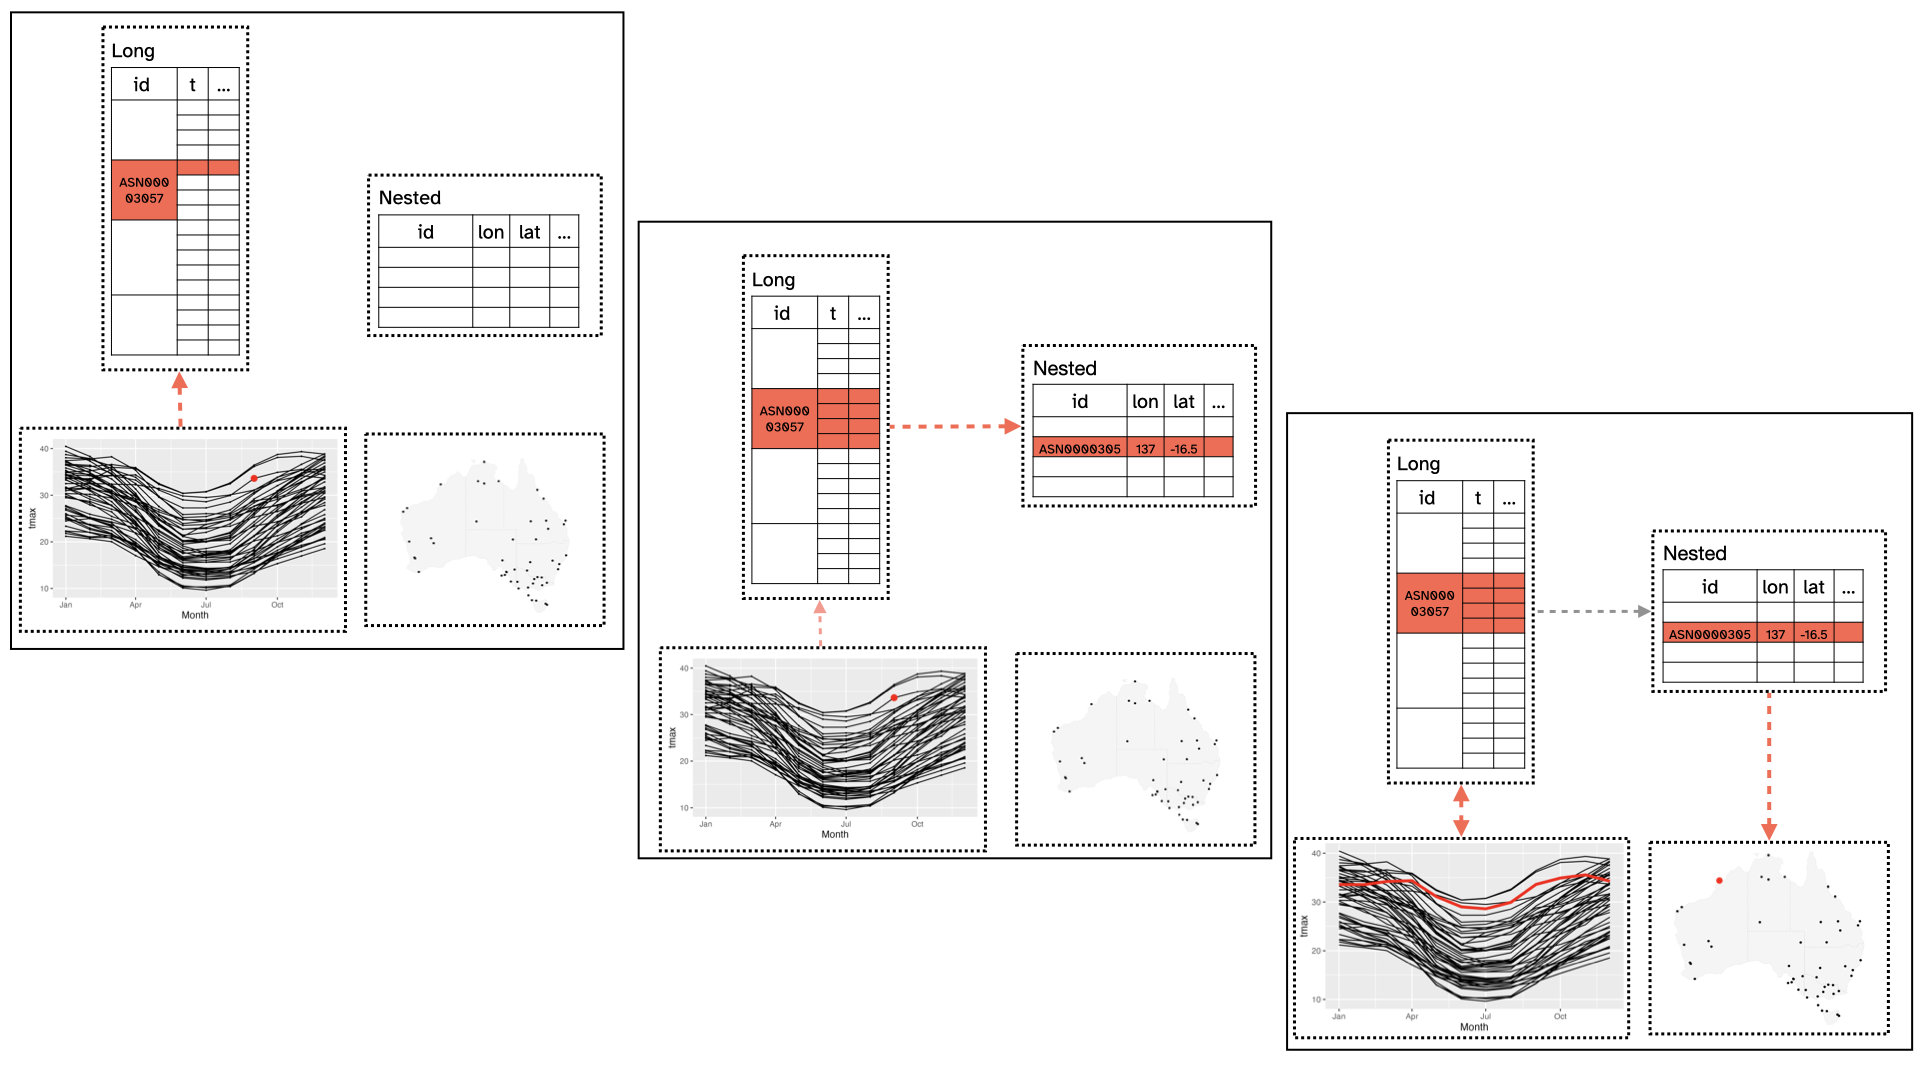
\includegraphics[width=1\linewidth,height=0.4\textheight]{/Users/sherryzhang/Documents/research/paper-cubble/figures/diagram-keynotes/diagram-keynotes.005} 

}

\caption{An illustration of the data model under interactive graphics with cubble. When a point on the time series is selected, the corresponding row in the long cubble will be activated. This will link to all the rows with the same id in the long cubble and the row in the nested cubble with the same id (middle). Both plots will be updated with the full line selected and the point highlighted on the map (right).}\label{fig:illu-interactive-2}
\end{figure}

\newpage

\hypertarget{refs}{}
\begin{CSLReferences}{1}{0}
\leavevmode\vadjust pre{\hypertarget{ref-leafpop}{}}%
Appelhans, Tim, and Florian Detsch. 2021. \emph{\pkg{leafpop}: Include Tables, Images and Graphs in Leaflet Pop-Ups}. \url{https://CRAN.R-project.org/package=leafpop}.

\leavevmode\vadjust pre{\hypertarget{ref-bach_review_2014}{}}%
Bach, Benjamin, Pierre Dragicevic, Dragicevic Archambault, Christophe Hurter, and Sheelagh Carpendale. 2014. {``A {Review} of {Temporal} {Data} {Visualizations} {Based} on {Space}-{Time} {Cube} {Operations}.''} \emph{Eurographics Conference on Visualization}, 19. \url{https://hal.inria.fr/hal-01006140/}.

\leavevmode\vadjust pre{\hypertarget{ref-buja1988elements}{}}%
Buja, Andreas, Daniel Asimov, and Catherine Hurley. 1988. {``Elements of a Viewing Pipeline.''} \emph{Dynamic Graphics Statistics}, 277.

\leavevmode\vadjust pre{\hypertarget{ref-buja1996interactive}{}}%
Buja, Andreas, Dianne Cook, and Deborah F Swayne. 1996. {``Interactive High-Dimensional Data Visualization.''} \emph{Journal of Computational and Graphical Statistics} 5 (1): 78--99. \url{https://doi.org/10.2307/1390754}.

\leavevmode\vadjust pre{\hypertarget{ref-cheng2016enabling}{}}%
Cheng, Xiaoyue, Dianne Cook, and Heike Hofmann. 2016. {``Enabling Interactivity on Displays of Multivariate Time Series and Longitudinal Data.''} \emph{Journal of Computational and Graphical Statistics} 25 (4): 1057--76. \url{https://doi.org/10.1080/10618600.2015.1105749}.

\leavevmode\vadjust pre{\hypertarget{ref-cocchi2019data}{}}%
Cocchi, Marina. 2019. \emph{Data Fusion Methodology and Applications}. Elsevier.

\leavevmode\vadjust pre{\hypertarget{ref-ctvspatiotemporal}{}}%
Edzer Pebesma, Roger Bivand. 2022. {``{CRAN} Task View: Handling and Analyzing Spatio-Temporal Data.''} \url{https://CRAN.R-project.org/view=SpatioTemporal}.

\leavevmode\vadjust pre{\hypertarget{ref-hersbach2020era5}{}}%
Hersbach, Hans, Bill Bell, Paul Berrisford, Shoji Hirahara, András Horányi, Joaquín Muñoz-Sabater, Julien Nicolas, et al. 2020. {``The Era5 Global Reanalysis.''} \emph{Quarterly Journal of the Royal Meteorological Society} 146 (730): 1999--2049.

\leavevmode\vadjust pre{\hypertarget{ref-ecwmfr}{}}%
Hufkens, Koen, Reto Stauffer, and Elio Campitelli. 2019. {``The \pkg{ecwmfr} Package: An Interface to ECMWF API Endpoints.''} \url{https://doi.org/10.5281/zenodo.2647541}.

\leavevmode\vadjust pre{\hypertarget{ref-lu_multidimensional_2018}{}}%
Lu, Meng, Marius Appel, and Edzer Pebesma. 2018. {``Multidimensional {Arrays} for {Analysing} {Geoscientific} {Data}.''} \emph{ISPRS International Journal of Geo-Information} 7 (8): 313. \url{https://doi.org/10.3390/ijgi7080313}.

\leavevmode\vadjust pre{\hypertarget{ref-mcintosh2018using}{}}%
McIntosh, Avery I, Helen E Jenkins, Laura F White, Marinus Barnard, Dana R Thomson, Tania Dolby, John Simpson, et al. 2018. {``Using Routinely Collected Laboratory Data to Identify High Rifampicin-Resistant Tuberculosis Burden Communities in the Western Cape Province, South Africa: A Retrospective Spatiotemporal Analysis.''} \emph{PLoS Medicine} 15 (8): e1002638.

\leavevmode\vadjust pre{\hypertarget{ref-michna2013rnetcdf}{}}%
Michna, Pavel, and Milton Woods. 2013. {``\pkg{RNetCDF}: A Package for Reading and Writing NetCDF Datasets.''} \emph{The R Journal} 5 (2): 29--36.

\leavevmode\vadjust pre{\hypertarget{ref-rnetcdf}{}}%
---------. 2021. \emph{\pkg{RNetCDF}: Interface to 'NetCDF' Datasets}. \url{https://CRAN.R-project.org/package=RNetCDF}.

\leavevmode\vadjust pre{\hypertarget{ref-spacetime}{}}%
Pebesma, Edzer. 2012. {``\pkg{spacetime}: Spatio-Temporal Data in r.''} \emph{Journal of Statistical Software} 51 (7): 1--30. \url{https://doi.org/10.18637/jss.v051.i07}.

\leavevmode\vadjust pre{\hypertarget{ref-stars}{}}%
---------. 2021. \emph{\pkg{stars}: Spatiotemporal Arrays, Raster and Vector Data Cubes}. \url{https://CRAN.R-project.org/package=stars}.

\leavevmode\vadjust pre{\hypertarget{ref-sf}{}}%
Pebesma, Edzer J. 2018. {``Simple Features for \proglang{R}: Standardized Support for Spatial Vector Data.''} \emph{R Journal} 10 (1): 439.

\leavevmode\vadjust pre{\hypertarget{ref-ncdf4}{}}%
Pierce, David. 2019. \emph{\pkg{ncdf4}: Interface to Unidata netCDF (Version 4 or Earlier) Format Data Files}. \url{https://CRAN.R-project.org/package=ncdf4}.

\leavevmode\vadjust pre{\hypertarget{ref-simmons2005ecmwf}{}}%
Simmons, Adrian, Mariano Hortal, Graeme Kelly, Anthony McNally, Agathe Untch, and Sakari Uppala. 2005. {``ECMWF Analyses and Forecasts of Stratospheric Winter Polar Vortex Breakup: September 2002 in the Southern Hemisphere and Related Events.''} \emph{Journal of the Atmospheric Sciences} 62 (3): 668--89. \url{https://doi.org/10.1175/JAS-3322.1}.

\leavevmode\vadjust pre{\hypertarget{ref-simmons2020global}{}}%
Simmons, Adrian, Cornel Soci, Julien Nicolas, Bill Bell, P. Berrisford, Rossana Dragani, Johannes Flemming, et al. 2020. {``Global Stratospheric Temperature Bias and Other Stratospheric Aspects of Era5 and Era5.1,''} no. 859 (January). \url{https://doi.org/10.21957/rcxqfmg0}.

\leavevmode\vadjust pre{\hypertarget{ref-stuart2010matching}{}}%
Stuart, Elizabeth A. 2010. {``Matching Methods for Causal Inference: A Review and a Look Forward.''} \emph{Statistical Science} 25 (1): 1.

\leavevmode\vadjust pre{\hypertarget{ref-tidync}{}}%
Sumner, Michael. 2020. \emph{\pkg{tidync}: A Tidy Approach to 'NetCDF' Data Exploration and Extraction}. \url{https://CRAN.R-project.org/package=tidync}.

\leavevmode\vadjust pre{\hypertarget{ref-sutherland2000orca}{}}%
Sutherland, Peter, Anthony Rossini, Thomas Lumley, Nicholas Lewin-Koh, Julie Dickerson, Zach Cox, and Dianne Cook. 2000. {``\pkg{Orca}: A Visualization Toolkit for High-Dimensional Data.''} \emph{Journal of Computational and Graphical Statistics} 9 (3): 509--29. \url{https://www.tandfonline.com/doi/abs/10.1080/10618600.2000.10474896}.

\leavevmode\vadjust pre{\hypertarget{ref-wang2020calendar}{}}%
Wang, Earo, Dianne Cook, and Rob J Hyndman. 2020. {``Calendar-Based Graphics for Visualizing People's Daily Schedules.''} \emph{Journal of Computational and Graphical Statistics} 29 (3): 490--502.

\leavevmode\vadjust pre{\hypertarget{ref-tidydata}{}}%
Wickham, Hadley. 2014. {``Tidy Data.''} \emph{Journal of Statistical Software} 59 (10): 1--23. \url{https://doi.org/10.18637/jss.v059.i10}.

\leavevmode\vadjust pre{\hypertarget{ref-ggplot2}{}}%
---------. 2016. \emph{Ggplot2: Elegant Graphics for Data Analysis}. Springer-Verlag New York. \url{https://ggplot2.tidyverse.org}.

\leavevmode\vadjust pre{\hypertarget{ref-tidyverse}{}}%
Wickham, Hadley, Mara Averick, Jennifer Bryan, Winston Chang, Lucy D'Agostino McGowan, Romain François, Garrett Grolemund, et al. 2019. {``Welcome to the {tidyverse}.''} \emph{Journal of Open Source Software} 4 (43): 1686. \url{https://doi.org/10.21105/joss.01686}.

\leavevmode\vadjust pre{\hypertarget{ref-dplyr}{}}%
Wickham, Hadley, Romain François, Lionel Henry, and Kirill Müller. 2022. \emph{Dplyr: A Grammar of Data Manipulation}. \url{https://CRAN.R-project.org/package=dplyr}.

\leavevmode\vadjust pre{\hypertarget{ref-Wickham2012-yr}{}}%
Wickham, Hadley, Heike Hofmann, Charlotte Wickham, and Dianne Cook. 2012. {``Glyph-Maps for Visually Exploring Temporal Patterns in Climate Data and Models.''} \emph{Environmetrics} 23 (5): 382--93.

\leavevmode\vadjust pre{\hypertarget{ref-knitr}{}}%
Xie, Yihui. 2015. \emph{Dynamic Documents with \proglang{R} and \pkg{knitr}}. 2nd ed. Boca Raton, Florida: Chapman; Hall/CRC. \url{https://yihui.name/knitr/}.

\leavevmode\vadjust pre{\hypertarget{ref-rmarkdown}{}}%
Xie, Yihui, J. J. Allaire, and Garrett Grolemund. 2018. \emph{R Markdown: The Definitive Guide}. Boca Raton, Florida: Chapman; Hall/CRC. \url{https://bookdown.org/yihui/rmarkdown}.

\leavevmode\vadjust pre{\hypertarget{ref-xie2014reactive}{}}%
Xie, Yihui, Heike Hofmann, and Xiaoyue Cheng. 2014. {``{Reactive Programming for Interactive Graphics}.''} \emph{Statistical Science} 29 (2): 201--13. \url{https://doi.org/10.1214/14-STS477}.

\end{CSLReferences}

\bibliographystyle{unsrt}
\bibliography{../references.bib}


\end{document}
